\documentclass[11pt,a4paper]{article}
%%%% BHAM PREAMBLE - SET THIS FIRST! %%%%
\newcommand{\bhamstudentname}{Binjie Zhang}
\newcommand{\bhamthesistitle}{Dynamical System State Prediction based on Generative Adversarial Network}
\newcommand{\bhamfronttitle}{Dynamical System State Prediction based on\\ Generative Adversarial Network}
\newcommand{\bhamschool}{School of Computer Science}
\newcommand{\bhamcollege}{Engineering and Physical Sciences}
\newcommand{\bhamdegree}{MSc. Advanced Computer Science}
\newcommand{\bhamid}{1870958}
\newcommand{\bhamsupervisor}{Dr Per Kristian Lehre}
\newcommand{\bhamyear}{2019}
%%%%           %%%%

\newcommand{\HRule}{\rule{\linewidth}{0.5mm}}
\renewcommand{\headrulewidth}{0pt}
\newcommand{\tab}{\hspace*{1.25em}}
\newcommand{\minitab}{\hspace*{0.25em}}
\usepackage[utf8]{inputenc}
\usepackage{graphics}
\usepackage{amsmath}
\usepackage{algorithm}
\usepackage{algorithmic}
\usepackage{amsthm}
\usepackage{graphicx}
\usepackage{subfigure}
\usepackage{multirow}
% \newenvironment{Declaration}{
% 	\begin{center}\normalfont\bfseries Declaration\end{center}
% 	\begin{quote}\par
% }
% {\end{quote}}

\usepackage{titling}	
\setlength{\droptitle}{-2.75cm}   % This is your set screw\\
\usepackage{titlesec}
\titleformat*{\section}{\normalsize	\bfseries}
\titleformat*{\subsection}{\small \bfseries}
\titleformat*{\subsubsection}{\footnotesize \bfseries}
%modifies the size of the gaps between the top of the title and bottom
% arguments {type}{left}{top}{bottom}
\titlespacing*{\section} {0pt}{3ex plus 1ex minus .2ex}{2ex plus .2ex}
\titlespacing*{\subsection} {0pt}{2.25ex plus 1ex minus .2ex}{0.75ex plus .2ex}
\titlespacing*{\subsubsection}{0pt}{2.ex plus 1ex minus .2ex}{0.5ex plus .2ex}


% \title{Dynamical System State Prediction based on Generative Adversarial Network}
% \author{Binjie Zhang}


\usepackage{natbib}
\usepackage{graphicx}

\begin{document}
\thispagestyle{empty}
\begin{titlepage}
\begin{center}
\begin{minipage}{6in}
  \centering
  \raisebox{-0.5\height}{
\includegraphics[width=1.25in]{crest}}
  \hspace*{.2in}
  \raisebox{-0.5\height}{
\includegraphics[height=0.9375in]{uni}}
  \end{minipage}
  \\ [1.0cm]
\textsc{{\LARGE \bhamschool\\}College of \bhamcollege}\\[3.5cm] 

\textsc{\Large MSc. Project}\\[0.5cm]

% Title
\HRule \\[0.4cm]
\begin{center}\Huge
\bhamfronttitle
\end{center}
\HRule \\[1.5cm]
% Team and Members

\begin{center}
Submitted in conformity with the requirements\\ for the degree of \bhamdegree\\
\bhamschool\\ University of Birmingham\\
\vspace{2cm}
Student name: \bhamstudentname\\
Student ID: \bhamid\\
Supervisor: \bhamsupervisor      
\end{center}
\vfill

% Bottom of the page
{\large September \bhamyear}

\end{center}
\end{titlepage}



\newpage
\thispagestyle{empty}
\begin{abstract}
Generative Adversarial Network has been widely concerned because of its extensive application ability and efficient training efficiency. However, most results of GAN application are meaningless at present. We hope to explore the more abilities of GAN and make more practical significance of GAN application results. Dynamical systems are often complicated, and there are rules behind the complex changes, sometimes the rules are simple, but challenging to solve. In this dissertation, we pay attention to whether GAN can be applied to predict the following states according to the current state of the dynamical system, so that we can use the neural network to solve problems without actually solving the rules behind the dynamical system. We first conducted a series of experiments to evaluate the training effect of GAN and then saved the generator in GAN for the prediction of dynamical system state. This project achieved a good implementation effect, indicating that GAN can be used to predict the following states based on the existing dynamical system states.
\\
\newline
    \textbf{Keywords:} Generative Adversarial Network, Dynamical system, prediction
\end{abstract}
\newpage
\thispagestyle{empty}
% \begin{Declaration}
% The material contained with this thesis has not previously been submitted for a degree at the University of Birmingham or any other university. The research reported within this thesis has been conducted by the author unless indicated otherwise.\\

% Signed: ..........................................................................................
% \end{Declaration}

\section*{Declaration}
The material contained within this report has not previously been submitted for a degree at the University of Birmingham or any other university. The research reported within this report has been conducted by the author unless indicated otherwise.\\

Signed: ....................................................................................................
\newpage
\thispagestyle{empty}
\tableofcontents
\newpage
\thispagestyle{empty}
\listoffigures
\listoftables
\newpage
\setcounter{page}{1}
\section{Introduction}
\subsection{Background}
Generative Adversarial Network (GAN)\citep{goodfellow2014generative} have become very popular because of their broad applicability in different fields. This concept was first proposed by Iain Goodfellow in 2014. Subsequently, many different scholars proposed many improved GAN based on the prototype of GAN and for different applications.
\\
\newline
GAN has received extensive attention in the field of computer vision since it was proposed. The main applications are focused on image synthesis and processing. In 2014, the initial effect of GAN could generate some blurred faces\citep{goodfellow2014generative}. In 2015, Radford proposed DCGAN, which combined the convolutional neural network with the generative adversarial network to produce a more realistic effect\citep{radford2015unsupervised}. In 2017, Tero Karras proposed Pro GAN. The key idea is to grow both the generator and discriminator progressively, speeding up the training and improve the stability, generated unprecedented high-quality images\citep{karras2017progressive}. Besides, GAN is also used in sequence generation to generate text or music. For example, C-RNN-GAN tries to learn and produce classical music\citep{mogren2016c}. Researchers in Insilico Medicine even proposed a method combining GAN and reinforcement learning for drug discovery\citep{putin2018adversarial}. In a word, GAN is widely used, but so far, the most result GAN produces is to generate some samples that look like the real ones. 
\\
\newline
The training process of the minimax game of GAN is innovative and efficient, and GAN should have great potential behind it to accomplish more meaningful things. The application results of GAN should have more practical significance, for example, it can be applied to some complex physical phenomena that are difficult to solve. Based on the training principle of GAN, we try to explore more potential abilities of GAN, make the result generated by GAN are more meaningful and practical. This is the motivation of this dissertation.
\\
\newline
A dynamical system is a fixed rule that describes how all points in a given space change over time. A dynamical system can describe many physical phenomena in nature and has a broad application value. Often, the differential equations of simple dynamical systems can sometimes be solved efficiently, for example, a simple pendulum system can be described by a second order differential equation with only one variable. Same as the pendulum, simple differential equations can describe many complex systems. However, for complex dynamical systems, it can be challenging to find differential equations which describe them. GAN can generate new samples based on learning with some existing samples. If the state of the dynamical system is taken as the input of the GAN network, will GAN network generate some similar states? Alternatively, can GAN predict the following states by learning the existing states? Based on the above questions, we propose the research problem of this dissertation, whether GAN can be used to predict the state of the dynamical system.
\\
\newline
\subsection{Research aim and objectives}
In the background, we mentioned the research question of this dissertation, whether GAN could be used to predict the state of the dynamical system. Precisely, whether the GAN can predict the following states by giving the states of the existing dynamical systems. The purpose of this dissertation is to explore the possibility of GAN predictive ability.
\\
\newline
To solve the research problem, we propose the following hypothesis:
\\
GAN can predict the state of the following dynamical system based on the state of the existing dynamical system. In this case, it can be further subdivided into using GAN to predict the state of simple dynamical systems and using GAN to predict the state of complex dynamical systems. Meanwhile, we also made a hypothesis that different topologies of GAN would affect the training effect on the same issue.
\\
In this dissertation, we hope to achieve the following research objectives:
\begin{itemize}
    \item Use differential equations to describe the motion state of the single pendulum model
    \item Use differential equations and other mathematical theorems to describe the motion state of the double pendulum model
    \item Improve GAN algorithm to suit for dynamical system prediction
    \item Conduct experiments to observe the influence of different topological structures on GAN training
    \item Conduct experiments to observe the predictive ability of GAN under different training iterations
    \item Use GAN to predict the motion state of single pendulum and double pendulum, and do visualization
    \item Analyse and discuss the results and draw conclusions
\end{itemize}
The structure of this dissertation is as follows. The first chapter is the background introduction, and the second chapter is the literature review, which briefly introduces the basic principles of GAN and dynamical system. The third chapter introduces the model of the dynamical system; GAN algorithm improved for the specific model and some relative knowledge. Chapter 4 will introduce experimental design and experimental results. The fifth chapter will discuss implementation and experiments. The final chapter will summarize the entire project.
\newpage
\section{Literature Review}
In order to apply GAN in the prediction of the dynamical system state, we need to know the basic methods of GAN and the basic concepts of the dynamical system. In this chapter, we will summarize the basic concepts of GAN, the objective function used and some applications through literature review. Then we will also briefly introduce the concepts of dynamic systems and traditional systems control theory used to solve the concept of dynamic systems.
\subsection{Generative adversarial network}
\subsubsection{Basic concept of GANs}
It can be seen by its name, Generative Adversarial Network is a generative model that learns the data distribution according to the existing data distribution through confrontation. The so-called confrontation process is because GAN does not use maximization possibility but introduces the concept of adversarial learning between generator and discriminator, i.e. generator and discriminator are two neural networks, the generator to is trying to generate realistic samples as much as possible, while the discriminator is trying to distinguish a sample is the real samples or the false samples generated by generator.
\\
\begin{figure}[ht!]
\centering
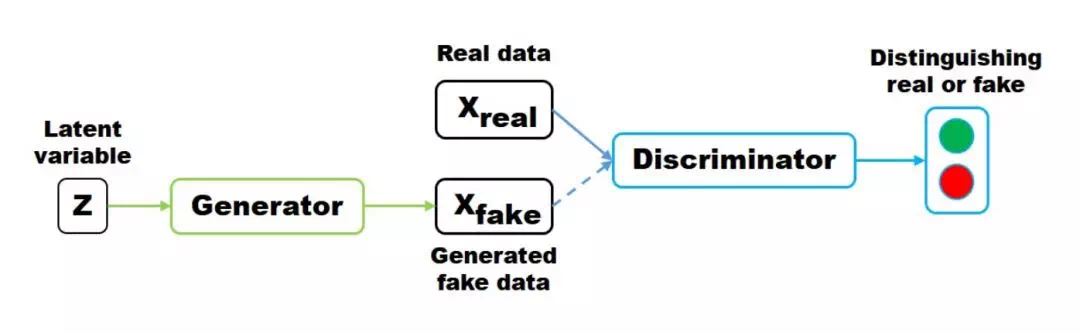
\includegraphics[scale=0.3]{1.png}
\caption{Generative Adversarial Network\citep{hong2019generative}}
\label{fig:GAN}
\end{figure}
\\
The learning process of GAN is shown in Figure 1. Generally speaking, the latent variable z is random Gaussian noise. After the latent variable z passes the generator, the generator generates a fake sample $Xfake$. Meanwhile, the input data of the discriminator can be either an $Xfake$ generated by the generator or an $Xreal$ from a real sample. The function of the discriminator is to identify whether the input sample is a real sample or a fake sample. In the Generative Adversarial Network\citep{goodfellow2014generative}, the optimization objective function used is:
\\
\newline
$$\min _{G} \max _{D} V(G, D)=\min _{G} \max _{D} \mathbb{E}_{x \sim p_{\text {data }}}[\log D(x)]+\mathbb{E}_{z \sim p_{x}}[\log (1-D(G(z))]$$
\\
\newline
This objective function is a minimax game. For the discriminator, it is facing a binary classification problem, namely discern between real and fake questions. $V (G, D)$ is the cross-entropy loss of the binary classification problem\citep{mao2017least}. So for generator $G$, in order to fool discriminator $D$ into thinking that the sample it generates is a real sample, we need to maximize the probability $D(G(z))$, which is to minimize $\log (1-D(G(z))$. It is worth noting that since the $\log(D(x))$ term is independent of the generator $G$, it can be ignored during the calculation. 
\\
\newline
During the training, generator $G$ and discriminator $D$ adopt the mode of alternating training. Firstly, the generator $G$ is fixed to train discriminator $D$, so that discriminator $D$ has certain discriminating ability at the early stage of training, Then fix discriminator $D$, train generator $G$, improve the generating ability of generator $G$, and keep repeating. What is interesting here is that for the generator $G$, minimize $\max _{D} V(D, G)$ is minimize the maximum value of $V (G, D)$. In order to ensure the maximum value of $V (D, G)$, in Goodfellow's algorithm, the discriminator is trained to iterate $k$ times, and the generator is iterated once. However, in experiments and practices, the value of $k$ is usually 1. When the generator $G$ is fixed, the optimal discriminator $\mathrm{D}^{*}(\mathrm{x})$ can be obtained by differentiating $V (D, G)$: $D^{*}(x)=\frac{p_{g}(x)}{p_{g}(x)+p_{d a t a}(x)}$. Then put the optimal discriminator $\mathrm{D}^{*}(\mathrm{x})$ into the above objective function, and then get the objective function of the generator equivalent to optimize the Jensen Shannon(JS) Divergence of $P_{data}(x)$ and $P_{g}(x)$ in the case of the optimal discriminator. JS divergence is a measure to measure the similarity of two distributions. For specific explanation, please refer to appendix B.
\\
\newline
It can be proved that the generation model will converge, and a state of equilibrium will be reached when the capacity of generator G and discriminator D is sufficient. At this point, $P_{data}(x)=Pg(x)$, and the discriminator's discriminant probability is $1/2$ for both the samples sampled in $P_{data}(x)$ and $P_{g}(x)$, which means that it is difficult for the discriminator to distinguish the generated sample from the real sample\citep{goodfellow2014generative}.
\\
\newline
\subsubsection{Objective function}
The objective function mentioned above is to minimize the JS divergence of two distributions. In addition to JS divergence, there are many ways to measure the distance between two distributions. Different objective functions can be obtained by defining different distance measures. In many methods to improve the stability of GAN training, distance measurement methods between different distributions are defined, such as LSGAN\citep{mao2017least} and WGAN\citep{arjovsky2017wasserstein}.
\\
\newline
LSGAN uses the following loss function:
\\
\newline
$$
\min _{D} J(D)=\min _{D}\left[\frac{1}{2} \mathrm{E}_{x \sim p_{\text {data}}(x)}[D(x)-a]^{2}+\frac{1}{2} \mathrm{E}_{z \sim p_{z}(z)}[D(G(z))-b]^{2}\right]
$$
\\
\newline
In this paper, $a=c=1$ and $b=0$. The author mentioned that LSGAN has two advantages compared with GAN. One is stable training, which solves the gradient saturation problem in the traditional GAN training process. Traditional GAN uses sigmoid cross-entropy as the loss\citep{goodfellow2014generative}. When the input is large, the gradient is 0. It is easy for the input of cross-entropy loss to appear gradient saturation, while LSGAN uses least square loss, which gradient saturation will not happen. Another advantage is the improved quality of the generation, which is achieved by punishing the generated samples far from the decision boundary of the discriminator\citep{mao2017least}.
\\
\newline
In WGAN, Martin Arjovsky proposes a new distance measurement method, Wasserstein distance, which is defined as follows:
\newline
$$
W\left(P_{data}, P_{g}\right)=\inf _{\gamma \sim \Pi\left(P_{data}, P_{g}\right)} \mathbb{E}_{(x, y) \sim \gamma}[\|x-y\|]
$$
\\
$\Pi\left(P_{data}, P_{g}\right)$ represents a combined distribution, and the marginal distribution of any distribution $\gamma$ in this group is $P_{data}(x)$ and $P_{g}(x)$. Intuitively, the probability distribution function (PDF) can be considered as the weight of the random variable at each point, so $W\left(P_{data}, P_{g}\right)$ represents the minimum amount of work required to move the probability distribution $P_{data} (x)$ to $P_{g} (x)$. The theory of WGAN is complicated, but it is easy to implement in code. The changes required are as follows:
\begin{itemize}
    \item Sigmoid is removed from the last layer of the discriminator
    \item Do not take log to the loss of generator and discriminator 
    \item After updating the parameters of the discriminator, their absolute values are truncated to no more than a fixed constant c. In the subsequent improvement of WGAN-GP\citep{gulrajani2017improved}, the author replaces gradient truncation with gradient penalty.
\end{itemize}{}
\subsubsection{Training difficulties of GANs}
In the paper of Goodfellow, there are two kinds of loss in the discriminator:
\newline
\begin{equation}
\mathbb{E}_{x \sim p_{g}}[\log (1-D(x))]
\end{equation}
\begin{equation}
\mathbb{E}_{x \sim p_{g}}[-\log (D(x))]
\end{equation}
\newline
The problem of equation (1) is when the discriminator reaches the optimal value, it is equivalent to minimizing the JS divergence between the generated distribution and the real distribution. However, since it is difficult to overlap the generated distribution with the real distribution and JS divergence has a mutation property, the generator will face the problem of gradient disappears.
\\
\newline
The problem of equation (2) is when the discriminator reaches the optimal value, it is equivalent to minimize the KL divergence directly generated from the real distribution and maximize their JS divergence, which are contradictory with each other, resulting in unstable gradient. Moreover, the asymmetry of KL divergence makes the generator prefer to lose its diversity rather than its accuracy, leading to mode collapse.
\\
\newline
To solve the problem of mode collapse, the objective function can be improved. In order to avoid the problem of mode hopping due to the optimization of maxmin, UnrolledGAN\citep{Metz2016unrolled} adopts the modification of generator loss to solve it. When UnrolledGAN updates the generator, it updates the generator for k times. The loss referred to is not the loss of a specific time, but the loss of k subsequent iterations of the discriminator. It is worth noting that the discriminator does not update its parameters for the next k iterations, but computes loss for the update generator. This approach allows the generator to take into account the subsequent k discriminator changes, thus avoiding the mode collapse caused by switching between different modes.
\subsubsection{Application of GANs}
\paragraph{Image processing}
In the field of image processing, the main application of GAN is image translation. Image translation is the transformation from one image (source domain) to another image (target domain). In the process of image translation, the content of the source domain image is kept unchanged, but the image style or some other attributes are converted into the target domain image. In terms of image translation, it can be divided into paired domain data translation and unpaired two domain data translation.
\\
\newline
Pix2pix\citep{isola2017image} is a typical example of paired domain data translation. Pix2pix uses paired data to train a conditional GAN, and the loss includes the loss of GAN and the loss of pixel-by-pixel difference. In contrast, PAN\citep{wang2018perceptual} uses the pixel-by-pixel difference in the feature graph as the perception loss to replace the pixel-by-pixel difference in the image to generate an image that is closer to the source domain in human eye perception.
\\
\newline
CycleGAN\citep{zhu2017unpaired} is a typical example of the problem of unpaired two domain data translation. CycleGAN uses two GAN pairs to convert the data of the source domain to the target domain through one GAN network and then uses another GAN network to convert the data of the target domain back to the source domain. The converted data and the source domain data happen to be in pairs, forming supervision information.
\paragraph{Sequence generation}
Compared with GAN's extensive application in image field, GANs are applied less often to text and voice problems. The main reason is that the speech data are discrete, and GAN uses backpropagation algorithm in the optimization process. For discrete values, GAN cannot directly jump to the target value, but can only approach step by step according to the gradient\citep{rocca_rocca_2019}. Another reason is that for the sequence generation problem, every time a word is generated, we need to determine whether the sequence is reasonable or not. It is difficult for the discriminator in GAN to achieve such a function.
\\
\begin{figure}[ht!]
\centering
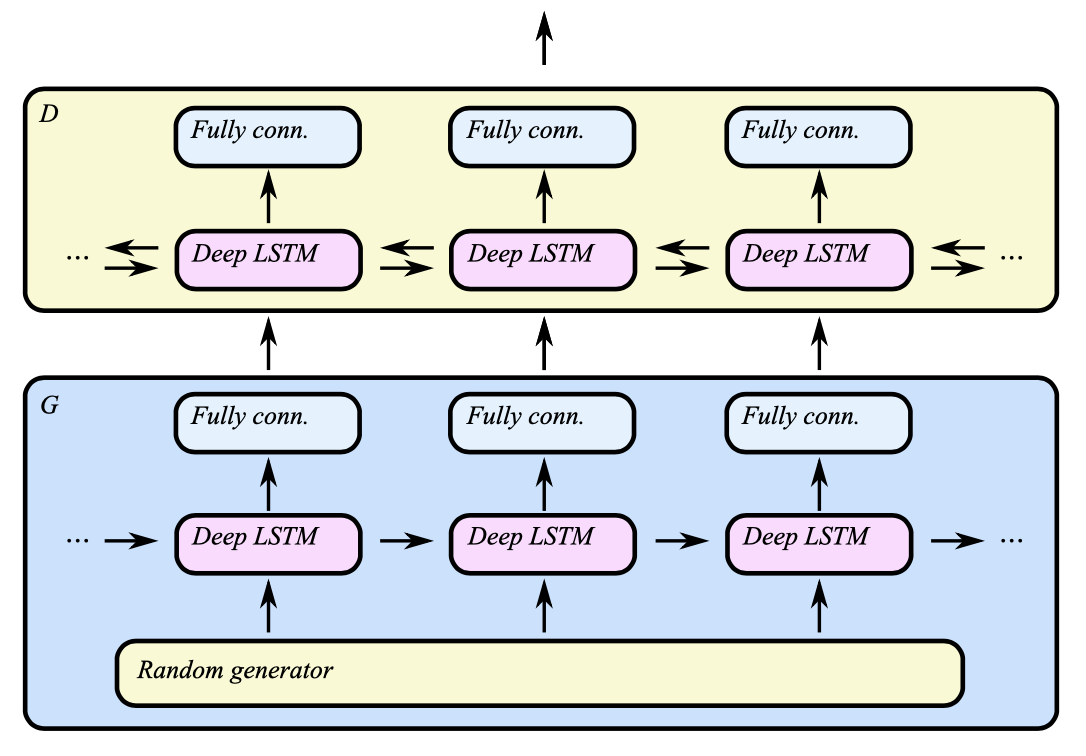
\includegraphics[scale=0.5]{2.png}
\caption{C-RNN-GAN\citep{mogren2016c}}
\label{fig:C-RNN-GAN}
\end{figure}
\\
\newline
However, GAN still has some applications in the field of sequence generation. For example, C-RNN-GAN\citep{mogren2016c} uses LSTM (Long Short-Term Memory) as generator and discriminator to directly generate the entire audio sequence. SeqGAN\citep{yu2017seqgan} uses policy gradient descent in reinforcement learning, takes the output of generator as an agent's strategy, and the output of discriminator as a reward then uses the policy gradient descent to train the model. ORGAN\citep{guimaraes2017objective}, based on SeqGAN, sets specific objective functions for specific goals.
\subsubsection{Advantages and disadvantages of GANs}
As a recently popular and widely used generative model, GAN has apparent advantages. For example, GAN can generate data in parallel because GAN does not need sampling but uses the generator to generate. Also, GAN does not need to introduce a lower bound to approximate likelihood. Because of the difficulty in optimization, VAE\citep{doersch2016tutorial} introduces variational lower bound to optimize likelihood. However, VAE made assumptions about the prior and posterior distributions, making it difficult for VAE to approach its variational lower bound; In practice, GAN generated results are much more precise than VAE.
\\
\newline
The shortcomings of GAN are also prominent. The main problem is unstable training. To solve this problem, WGAN and LSGAN have adopted different methods. Another drawback is that patterns are prone to collapse. Although there are many related studies, this problem has not been completely solved due to the high dimensional nature of image data.
\subsection{Dynamical system}
In mathematics, a dynamical system is a function that describes the time dependence of a point in geometric space. It is mainly used to describe complex dynamical systems, which are generally expressed by differential equations or difference equations. In terms of differential equations, time is continuous, and such systems are called "continuous dynamical systems". In terms of difference equations, states of systems are examined at a series of discrete time points, such systems are called "discrete dynamical systems". In a dynamical system, the state is a real number that can be determined, and the corresponding state will change slightly at different time points. The evolution rule of the dynamical system is a fixed rule of a set of functions, which describes how the future state changes from the current state. This rule is generally deterministic.
\\
\newline
A dynamical system can be divided into linear dynamical system and nonlinear dynamical system. The linear dynamical system evolves according to fixed rules, and the linear superposition of any two solutions of the system equation is still a solution of the equation. However, the nonlinear dynamical system does not meet the superposition principle, and there will be random and unpredictable conditions, which is called chaotic system\citep{arrowsmith1990introduction}.

\subsubsection{Control theory}
Control theory mainly deals with dynamical systems with input signals. Modern control theory uses state space representation in time domain to express the relationship between input, output and state variables in the system by first-order differential equations. To abstract the number of inputs, outputs, and state variables, these variables are typically represented as vectors, while differential equations or algebraic equations are represented as matrices. State space representation, also known as time domain analysis, provides a convenient and concise way to model and analyse systems with multiple inputs and outputs. In the case of inputs and outputs, Laplace transforms can also be used to include all the data of the system\citep{lee1967foundations}.
\\
\begin{figure}[ht!]
\centering
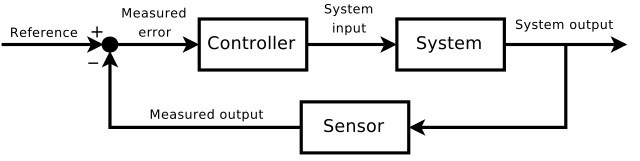
\includegraphics[scale=0.4]{3.png}
\caption{Control theory}
\label{fig:Control theory}
\end{figure}
\\
\subsection{Related work}
Generally speaking, dynamical system problems can be solved by system control theory, but for complex dynamical systems, system control theory does not have an excellent performance. So, we try to use adversarial neural network to predict dynamic system state. However, there are not many applications in dynamic system state prediction.
\\
\newline
Wu wrote a paper about enforcing statistical constraints in GAN to solve the partial differential equations in simulating complex physical systems\citep{wu2019enforcing}.It also shows that the statistical regularization performs better than traditional GANs.
\\
\newline
Due to the confidentiality of real phasor measurement unit (PMU) data and the fact that the infrastructure information of real power system cannot be publicly accessed, Zheng proposed a model-free method to generate synthetic PMU data directly. Instead of building a synthetic power grids, they used real PMU data to train generative adversarial network and then generated synthetic PMU measurement data through time simulation. This work is the first attempt to use a generative model to generate real system data\citep{zheng2018synthetic}.
\\
\newline
Li et al. proposed the anomaly detection with GAN for multivariate time series in large and complex cyber-physical systems\citep{li2018anomaly}, they also named a new type of GAN which is MAD-GAN\citep{li2019mad}.
\newpage
\section{Approach}
There are many different kinds of dynamical systems, and different dynamical systems have different characteristics. In this dissertation, we choose the pendulum model as the primary research object. Pendulum model can be divided into the single pendulum and double pendulum, the simple pendulum is a relatively simple model, and the law of its motion state is evident. However, the double pendulum is a very complex dynamical system model, and the motion state is not regular, easy to produce chaos phenomenon. Therefore, single pendulum and double pendulum models can well represent simple and complex dynamical system models. This chapter will mainly introduce the mathematical solution of the motion state of the single pendulum and double pendulum, and the improvement of GAN algorithm for specific problems.
\subsection{Single pendulum}
The pendulum is a device that can produce reciprocating swing. One end of a thin rod without weight or a thin, flexible rope that cannot be extended is suspended at a fixed point in the gravity field, and the other end is consolidated with a heavy ball to form a single pendulum. If the ball oscillates only in the vertical plane, it is a plane pendulum. The single pendulum is a simple dynamical system. The state of the pendulum can be expressed by the velocity at the current moment and the angular between the rope and the vertical plane.
\\
\begin{figure}[ht!]
\centering
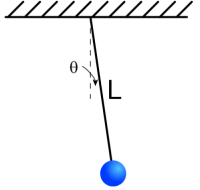
\includegraphics[scale=0.8]{4.png}
\caption{Single pendulum}
\label{fig:Single pendulum}
\end{figure}
\\
According to Newton's laws of mechanics, the simple pendulum angular function of time can be described as follows.
\\
\newline
First, the gravitational torque of the single pendulum is:
\begin{equation}
M=-m g l \sin \theta
\end{equation}
where $m$ is the mass, $g$ is the acceleration of gravity, $l$ is the length of the pendulum, and $\theta$ is the angle of the pendulum with the vertical direction.
\\
\newline
From the angular momentum theorem,
\begin{equation}
M=I \beta
\end{equation}
where $I$ is the moment of inertia of a pendulum and $\beta$ is angular acceleration.
\begin{equation}
I=m \cdot l^{2}
\end{equation}
\begin{equation}
\beta=\frac{d^{2} \theta}{d t^{2}}
\end{equation}
simplify to:
\begin{equation}
\frac{d^{2} \theta}{d t^{2}}+\frac{g}{l} \sin \theta=0
\end{equation}
The symbolic solution to this differential equation cannot be found directly, but python has built-in odeint functions that can be used to find numerical solutions to differential equations. Since odeint requires that each differential equation contain only the first derivative, the following deformation can be obtained.
\begin{equation}
\frac{d \theta(t)}{d t}=v(t)
\end{equation}
\begin{equation}
\frac{d v(t)}{d t}=-\frac{g}{\ell} \sin \theta(t)
\end{equation}
From the above two expressions, through the function odeint, we can find the state of a single pendulum. Figure 5 below shows the angular and velocity of a single pendulum at different times.
\\
\begin{figure}[h]
\centering
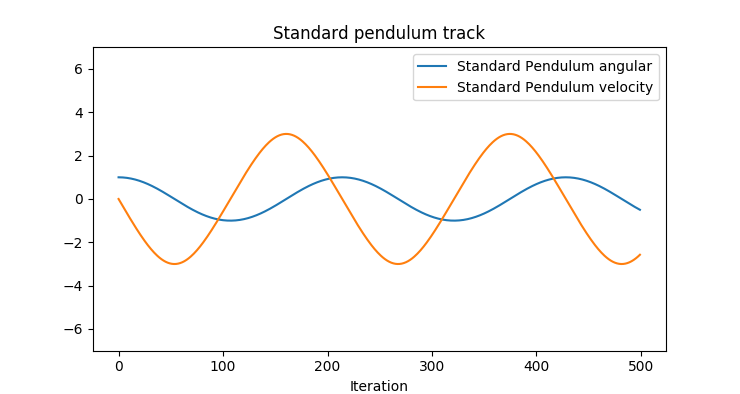
\includegraphics[scale=0.5]{6.png}
\caption{Standard single pendulum track}
\label{fig:Standard single pendulum track}
\end{figure}
\\
\subsection{Double pendulum}
Double pendulum is a system consisting of a single pendulum connected to the tail of another single pendulum. The double pendulum has both simple structure and complex behaviour. it is a simple dynamical system with chaotic properties.
\\
\begin{figure}[h!]
\centering
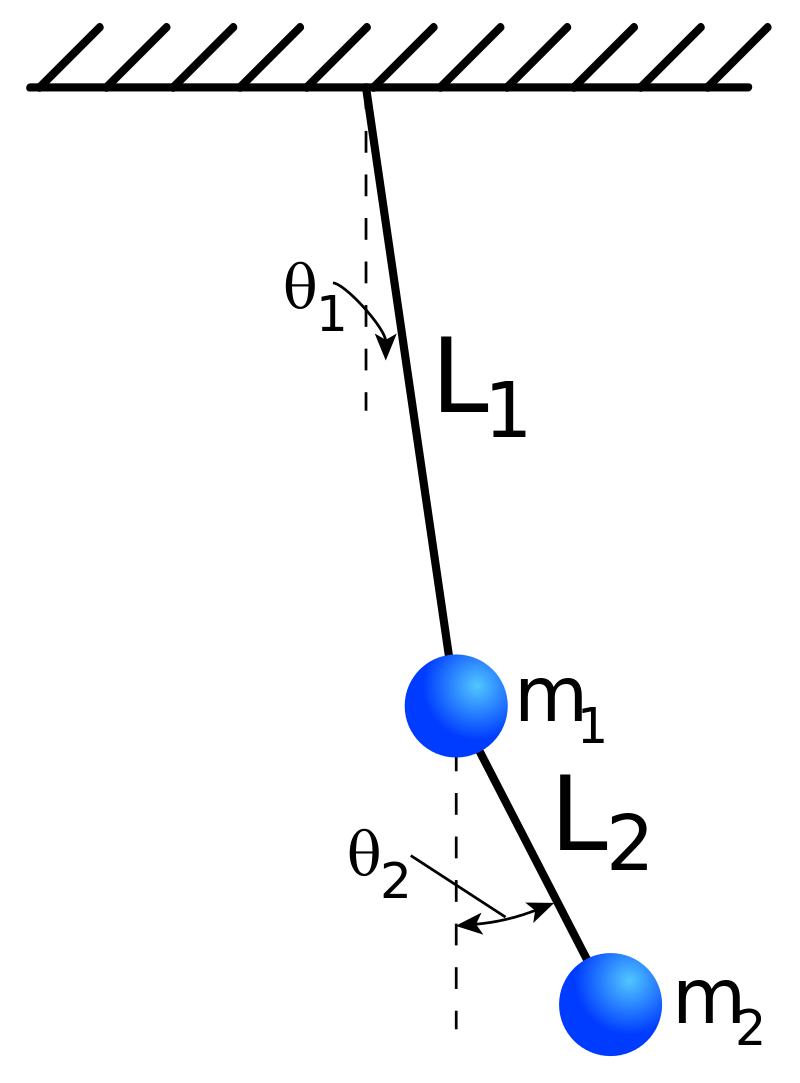
\includegraphics[scale=0.15]{5.png}
\caption{Double pendulum}
\label{fig:Double pendulum}
\end{figure}
\\
The differential equations of double pendulum system can be obtained by Lagrangian mechanics. Suppose the coordinates of the sphere connected by rod $L_{1}$ are $x_{1}$ and $y_{1}$, and the coordinates of the sphere connected by rod $L_{2}$ are $x_{2}$ and $y_{2}$, then the relationship between $x_{1}$ ,$y_{1}$ ,$x_{2}$ and $y_{2}$ and the two angles is as follows:
\begin{equation}
x_{1}=L_{1} \sin \left(\theta_{1}\right)
\end{equation}
\begin{equation}
y_{1}=-L_{1} \cos \left(\theta_{1}\right)
\end{equation}
\begin{equation}
x_{2}=L_{1} \sin \left(\theta_{1}\right)+L_{2} \sin \left(\theta_{2}\right)
\end{equation}
\begin{equation}
y_{2}=-L_{1} \cos \left(\theta_{1}\right)-L_{2} \cos \left(\theta_{2}\right)
\end{equation}
according to the formula of Lagrange quantity:
\begin{equation}
\mathcal{L}=T-V
\end{equation}
where $T$ is the kinetic energy of the system and $V$ is the potential potential energy of the system. Thus, the equation can be obtained as follows:
\begin{equation}
\mathcal{L}=\frac{m_{1}}{2}\left(\dot{x}_{1}^{2}+\dot{y}_{1}^{2}\right)+\frac{m_{2}}{2}\left(\dot{x}_{2}^{2}+\dot{y}_{2}^{2}\right)-m_{1} g y_{1}-m_{2} g y_{2}
\end{equation}
after substituting the above equation, we can get:
\begin{equation}
\begin{aligned} \mathcal{L}=\frac{m_{1}+m_{2}}{2} & L_{1}^{2} \dot{\theta}_{1}^{2}+\frac{m_{2}}{2} L_{2}^{2} \dot{\theta}_{2}^{2}+m_{2} L_{1} L_{2} \dot{\theta}_{1} \dot{\theta}_{2} \cos \left(\theta_{1}-\theta_{2}\right)+\\ &\left(m_{1}+m_{2}\right) g L_{1} \cos \left(\theta_{1}\right)+m_{2} g L_{2} \cos \left(\theta_{2}\right) \end{aligned}
\end{equation}
for $\theta_{1}$:
\begin{equation}
\frac{d}{d t} \frac{\partial \mathcal{L}}{\partial \dot{\theta}_{1}}-\frac{\partial \mathcal{L}}{\partial \theta_{1}}=0
\end{equation}
\begin{equation}
\begin{aligned} \left(m_{1}+m_{2}\right) L_{1} \ddot{\theta}_{1}+m_{2} L_{2} \cos \left(\theta_{1}-\theta_{2}\right) \ddot{\theta}_{2}+\\
m_{2} L_{2} \sin \left(\theta_{1}-\theta_{2}\right) \dot{\theta}_{2}^{2}+\left(m_{1}+m_{2}\right) g \sin \left(\theta_{1}\right)=0 \end{aligned}
\end{equation}
for $\theta_{2}$:
\begin{equation}
\frac{d}{d t} \frac{\partial \mathcal{L}}{\partial \dot{\theta}_{2}}-\frac{\partial \mathcal{L}}{\partial \theta_{2}}=0
\end{equation}
\begin{equation}
m_{2} L_{2}\left[L_{2} \ddot{\theta}_{2}+L_{1} \cos \left(\theta_{1}-\theta_{2}\right) \ddot{\theta}_{1}-L_{1} \sin \left(\theta_{1}-\theta_{2}\right) \dot{\theta}_{1}^{2}+g \sin \left(\theta_{2}\right)\right]=0
\end{equation}
Since the equation contains the second derivative, it is impossible to use odeint function for a numerical solution directly. Odeint requires that each differential equation only contains the first derivative, so it can be rewritten into the following four first-order differential equations.
\begin{equation}
\dot{\theta}_{1}=v_{1}
\end{equation}
\begin{equation}
\dot{\theta}_{2}=v_{2}
\end{equation}
\begin{equation}
\begin{aligned}\left(m_{1}+m_{2}\right) L_{1} \dot{v}_{1}+m_{2} L_{2} \cos \left(\theta_{1}-\theta_{2}\right) \dot{v}_{2}+\\
m_{2} L_{2} \sin \left(\theta_{1}-\theta_{2}\right) \dot{\theta}_{2}^{2}+\left(m_{1}+m_{2}\right) g \sin \left(\theta_{1}\right)=0 \end{aligned}
\end{equation}
\begin{equation}
L_{2} \dot{v}_{2}+L_{1} \cos \left(\theta_{1}-\theta_{2}\right) \dot{v}_{1}-L_{1} \sin \left(\theta_{1}-\theta_{2}\right) \theta_{1}^{2}+g \sin \left(\theta_{2}\right)=0
\end{equation}
The state of the double pendulum can be deduced from above. Figure 7 shows the angular and velocities of the two balls at different times.
\begin{figure}[ht!]
\centering
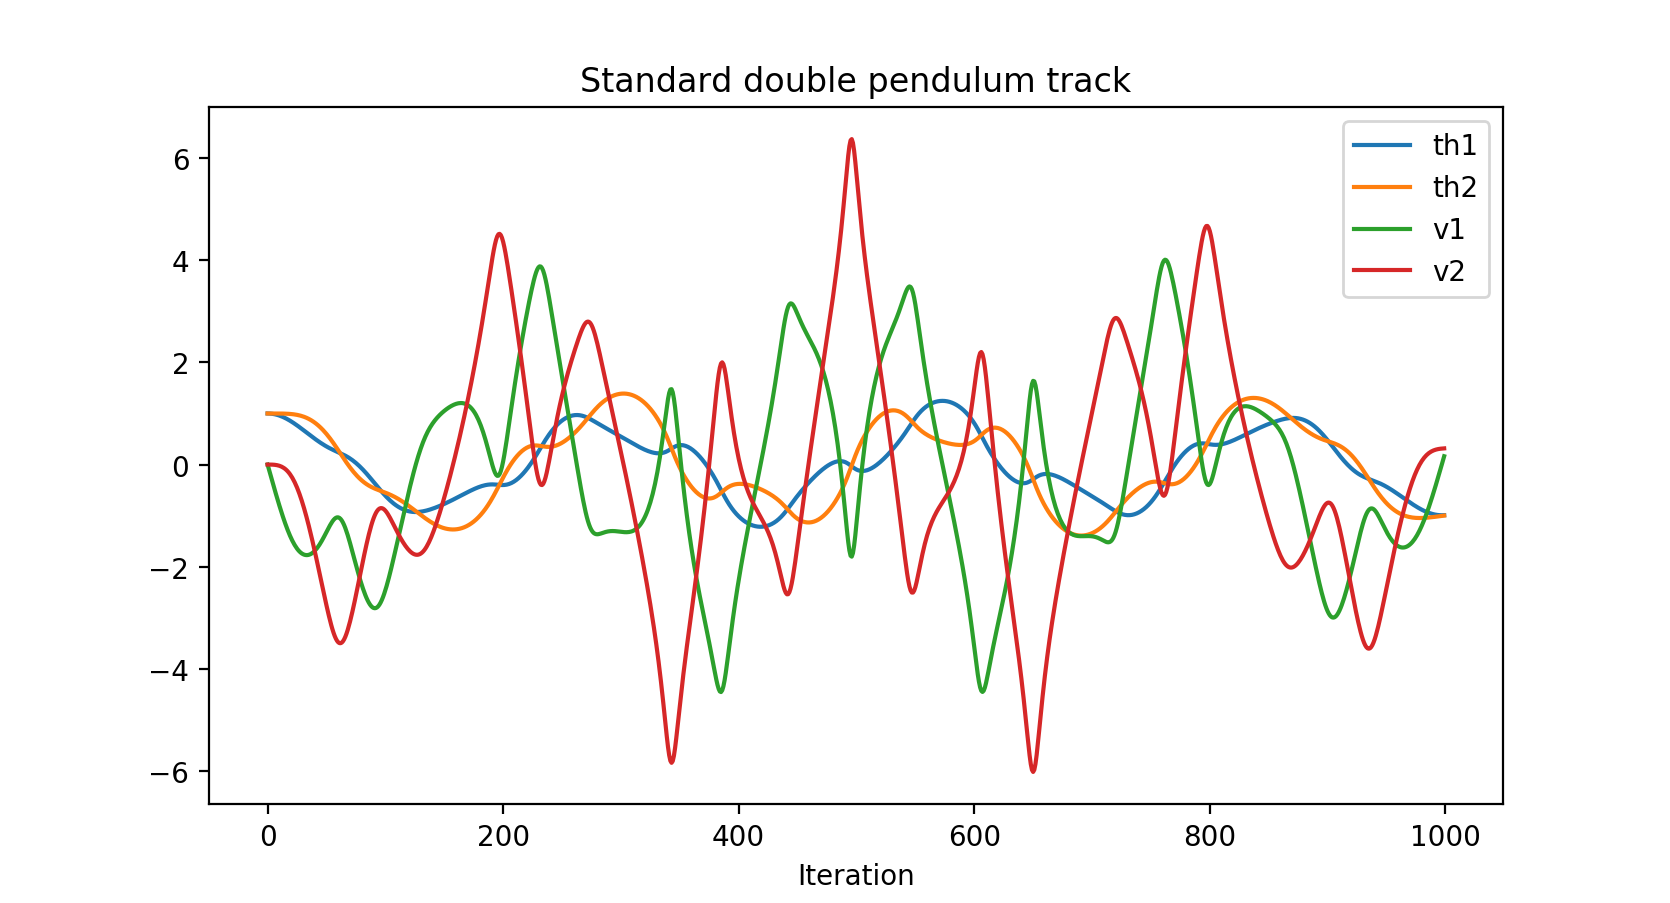
\includegraphics[scale=0.5]{7.png}
\caption{Standard double pendulum track}
\label{fig:Standard double pendulum track}
\end{figure}
\subsection{Improved algorithm}
Based on the original GAN algorithm of Goodfellow, the algorithm was modified for specific problems. The goal of this project is to use GAN to predict the state of dynamical systems. As mentioned in 3.1 and 3.2, the dynamical system used is the motion state of the single pendulum and double pendulum, specifically, the angular and velocity of the ball corresponding to a different time.
\\
\newline
Because this project needs to predict the next unknown motion state based on the known motion state, the input of the generator should be the known current state. We try to use the generator to predict the state of the next time corresponding to the current state from the known current state, so the input of the generator is the current state, not random input. After a generator generates a state, since a differential equation can solve the motion state of a single pendulum, each state generated by generator corresponds to a real state. The discriminator will distinguish from the corresponding real state and the state generated by the generator and optimize the discriminator's discriminating ability, and generator's generating ability through back propagation.
\\
\newline
The idea seems plausible since the states of a pendulum are generated on a fixed timeline; each state is theoretically corresponding to the timeline. However, in practical training, this one-to-one correspondence according to the time axis does not seem to be a good way to fix the order of pendulum states, and the discriminator will not know what the previous state corresponding to its input state is, so the discriminator may not learn any discriminating ability. At the beginning of the project, the reasons mentioned above are the reasons of GAN's weak training effect.
To solve this problem, we have made a few improvements to the input of the discriminator. We add the state generated by the generator, and the real state, to the previous state input by the generator to form a new vector of twice the length of the original input vector. The first half of the new input vector is the state at the current moment corresponding to each moment, and the second half is the state at the next moment corresponding to the corresponding state generated by the generator, or the real state at the next moment solved by the differential equation. After modifying the input of discriminator, GAN's learning and prediction effects become very obvious.
\\
\newline
The above two points are the improvement compared with the original algorithm, one is the modification of generator input, and the other is the modification of discriminator input. The specific algorithm is as follows.
\\
\newline
\begin{algorithm}[ht!]
\caption{Minibatch stochastic gradient descent training of generative adversarial nets for Pendulum. The number of steps to apply to the discriminator, $k$, is a hyperparameter.  I used $k = 1$, the least expensive option, in my experiments.}
\label{algorithm}
\begin{algorithmic}[1]
\STATE Sample $t$ continue time point \{$t^{(0)}$, $t^{(1)}$,…,$t^{(t-1)}$\} in the period of time $T$
\STATE Use ordinary differential equation produce t states \{$s^{(0)}$, $s^{(1)}$, …,$s^{(t-1)}$\} as $S$, each state include current angular and velocity [$\alpha$, $v$]
\FOR{number of training iterations}
\FOR{$k$ steps}
\STATE Sample minibatch of m states samples \{$s^{(0)}$, $s^{(1)}$, …,$s^{(m-1)}$\} as $C$ from $S$
\STATE For each state in C, move one bit forward \{$s^{(1)}$, $s^{(2)}$, …,$s^{(m)}$\}, indicating the next state corresponding to each state in $C$ as $C^{\prime}$
\STATE Obtaining generated m states \{$s^{(1^{\prime})}$, $s^{(2^{\prime})}$, …,$s^{(m^{\prime})}$\} as $G$ form Generator
\STATE Concatenate each state from $C$ and $C^{\prime}$ to \{$x^{(0)}$, $x^{(1)}$, …,$x^{(m-1)}$\} as $D_{real}$, each $x^{(i)}$ corresponding to[$s^{(i)}$, $s^{(i+1)}$]
\STATE Concatenate each state from $C$ and $G$ to \{$y^{(0)}$, $y^{(1)}$, …,$y^{(m-1)}$\} as $D_{fake}$, each $y^{(i)}$ corresponding to[$s^{(i)}$, $s^{(i+1)^{\prime}}$]
\STATE Update the discriminator by ascending its stochastic gradient:
$$
\nabla_{\theta_{d}} \frac{1}{m} \sum_{i=0}^{m}\left[\log D\left(x^{(i)}\right)+\log \left(1-D\left(y^{(i)}\right)\right]\right.
$$
\ENDFOR
\STATE Sample minibatch of m states samples \{$s^{(0)}$, $s^{(1)}$, …,$s^{(m-1)}$\} as $C$ from $S$
\STATE Update the generator by descending its stochastic gradient:
$$
\nabla_{\theta_{g}} \frac{1}{m} \sum_{i=0}^{m} \log \left(1-D\left(y^{(i)}\right)\right)
$$
\ENDFOR
\STATE The gradient-based optimizer is \textbf{Adam}.
\end{algorithmic}
\end{algorithm}
The flow chart of the improved algorithm is shown in Figure 8.
\begin{figure}[ht!]
\centering
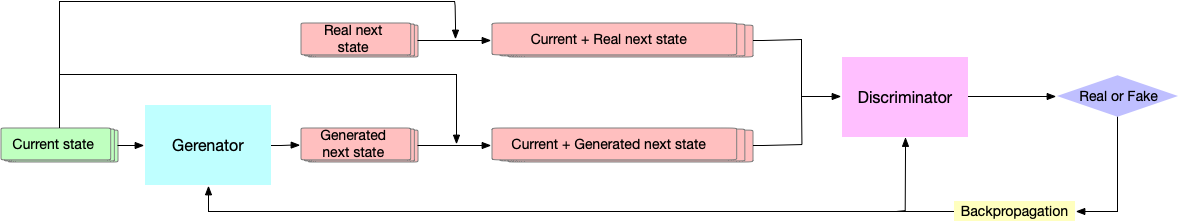
\includegraphics[scale=0.32]{8.png}
\caption{Flow chart of improved GAN}
\label{fig:Flow chart of improved GAN}
\end{figure}
\newpage
\subsection{Mean squared error}
In the experiment, the critical point is to evaluate the training effect of the GAN network. Since there is no verification set in the GAN training process, it is difficult to evaluate the training effect of the GAN intuitively. Because we can solve the real value of dynamical system state by a differential equation, we can compare the predicted result of GAN with the real value solved by differential equation and take the difference of the two values as the standard to judge the performance of GAN. Therefore, we add the mean squared error (MSE) as the standard to judge the performance of GAN. The smaller the mean squared error value is, the closer the predicted value is to the formal value, and the better the prediction ability of GAN for dynamical system is.
\\
\newline
In statistics, the mean squared error is a measure of the degree of difference between an estimator and a standard quantity, it is always non-negative, and values closer to zero are better. It is an estimation function $T$ for the unobservable parameter $\theta$, which is defined as:
$$
\operatorname{MSE}(T)=\mathrm{E}\left((T-\theta)^{2}\right)
$$
a more intuitive expression is:
$$
\mathrm{MSE}=\frac{1}{n} \sum_{i=1}^{n}\left(Y_{i}-\hat{Y}_{i}\right)^{2}
$$
\subsection{Activation function}
GAN’s generator and discriminator are two neural networks, we use the most common fully connected neural network. For the generator, there is an input layer, server hidden layers, and an output layer. The network structure of the discriminator is similar to that of the generator. However, there is a small difference. The function of the discriminator is to distinguish true and false, which can be regarded as a dichotomy problem. Every time the discriminator obtains an input, it corresponds to an output. The output value is between 0 and 1. The output value is close to 0, indicating that the discriminator determines that the current input is false; the output value is close to 1, indicating that the discriminator checks that the current input is true. In the implementation, we add a $sigmoid ()$ function to the output of the discriminator. This activation function is a logical function and is often used as a dichotomy problem. On the function definition, the domain of the sigmoid activation function can go to any range of real Numbers, returning values in the range of 0 to 1. The expression is as follows:
$$
S(x)=\frac{1}{1+e^{-x}}=\frac{e^{x}}{e^{x}+1}
$$
Figure 9 is the curve of sigmoid.
\begin{figure}[ht!]
\centering
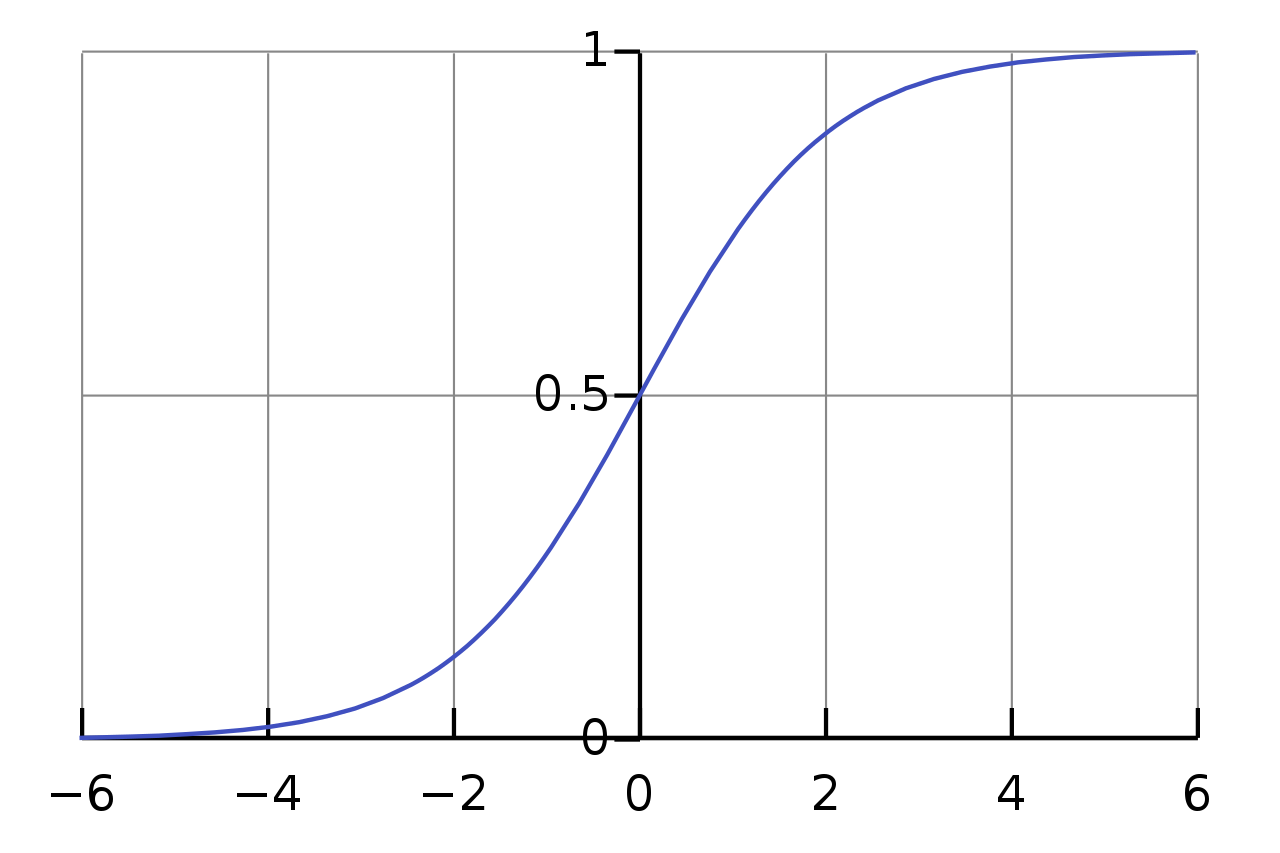
\includegraphics[scale=0.15]{9.png}
\caption{Curve of sigmoid}
\label{fig:Curve of sigmoid}
\end{figure}
\\
\newline
For the generator, in addition to the output layer, we give each layer Rectified Linear Unit(ReLU), $ReLU$ is a kind of common nonlinear excitation function. It is defined as:
$$
f(x)=\left\{\begin{array}{l}{x, \text { if } x>0} \\ {0, \text { if } x \leq 0}\end{array}\right.
$$
In the neural network, $ReLU$ as the activation function of neurons defines the nonlinear output results of neurons after linear transformation. Figure 10 is the curve of $ReLU$.
\begin{figure}[ht!]
\centering
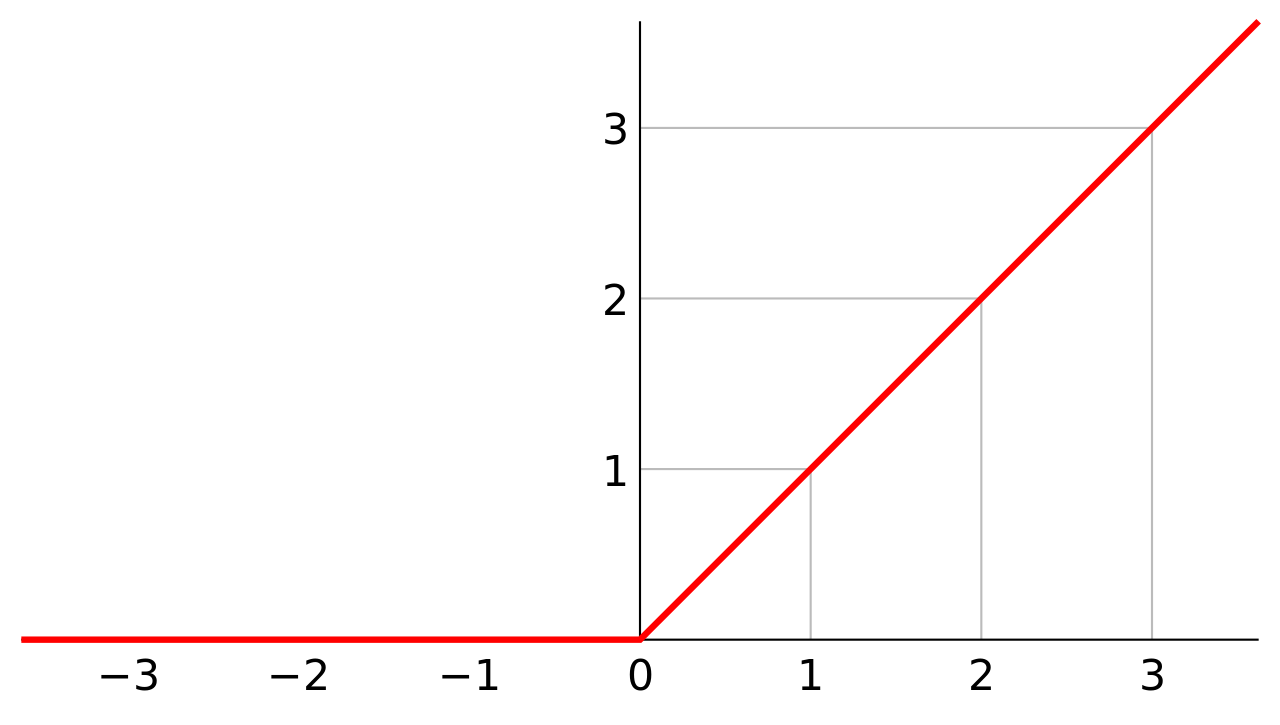
\includegraphics[scale=0.15]{10.png}
\caption{Curve of ReLU}
\label{fig:Curve of ReLU}
\end{figure}
\\
$ReLU$ is generally good at training, but it has its drawbacks. For input less than 0, the gradient of this neuron is always 0, and during training, it is easy to cause the death of the neuron. To solve this problem, the author proposed using $Leaky ReLU$ in the hidden layer of the discriminator in DCGAN\citep{radford2015unsupervised}. The gradient with Leaky linear rectifier function ($Leaky ReLU$) is a constant $\lambda \in(0,1)$ , not 0. When the input value is positive, the linear rectifier function with leakage is consistent with the ordinary slope function. $Leaky ReLU$ assigns a non-zero slope to all negative values when the input value is negative. This effectively avoids the problem of neuron death. The expression is: 
$$
f(x)=\left\{\begin{array}{l}{x, \text { if } x>0} \\ {\lambda x, \text { if } x \leq 0}\end{array}\right.
$$
Figure 11 is the curve of $Leary ReLU$.
\begin{figure}[ht!]
\centering
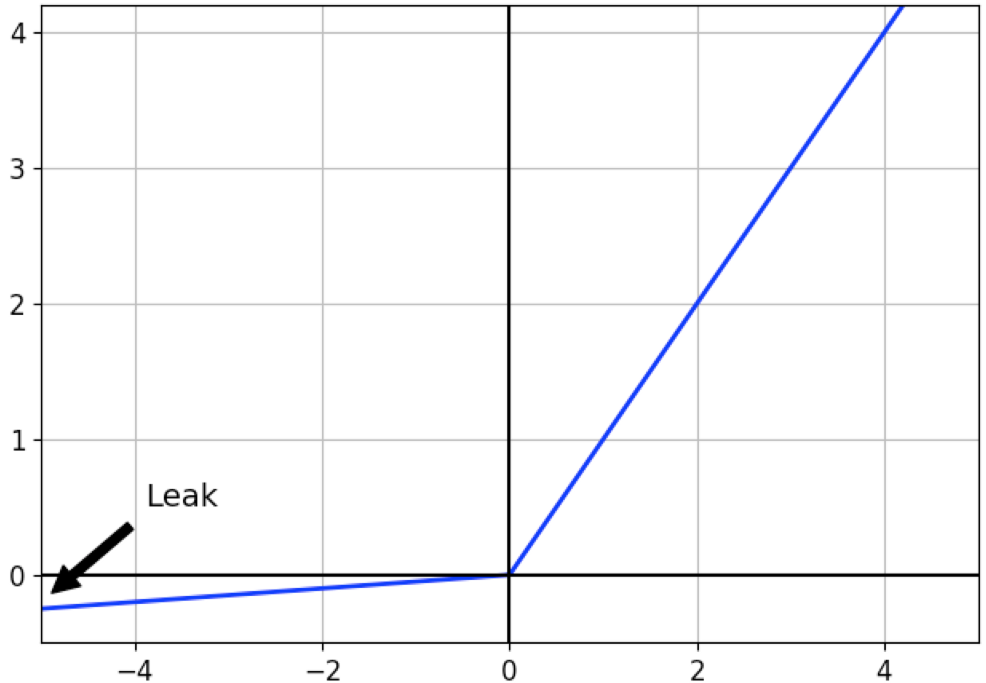
\includegraphics[scale=0.2]{11.png}
\caption{Curve of Leaky ReLU}
\label{fig:Curve of Leaky ReLU}
\end{figure}
\\
In conclusion, both $ReLU$ and $Leaky ReLU$ could make gradient descent and back propagation more productive and avoid the problem of gradient explosion and gradient disappearance. In this experiment, we used $ReLU$ in the generator and $Leaky ReLU$ in the discriminator.
\newpage
\section{Experiment and result}
The previous chapter introduces the dynamic system model selected in this project, single pendulum and double pendulum, and GAN algorithm based on specific problems. In this chapter, we will introduce the specific experimental contents. Since vectors represent the state of dynamical systems, we chose PyTorch as the training framework. It is based on the Python machine learning library, and its calculation is similar to the tensor calculation of NumPy.
\\
\subsection{Topological architecture}
\subsubsection{Number of neurons}
For neural networks, different topology and different Numbers of neurons will affect the performance of the whole neural network. In this part, we used the training pendulum to design the experiment and examined the effects of the different number of neurons and the different number of hidden layers on the training effect. Here, we use MSE to evaluate the training performance of GAN. 
\\
\newline
The first set of experiments is the influence of the different number of neurons on GAN performance under the same number of generator and discriminator network layers. In this experiment, there are four experimental groups, and the specific settings of the number of neurons in the four experimental groups are shown in Table 1. 
\begin{table}[ht]
\caption{Different number of neurons}
\vspace*{10pt}
\begin{tabular}{l|l|c|c|c|c}
\hline
                                   &                                                              & Group 1  & Group 2  & Group 3    & Group 4    \\ \hline
Generator                          & \begin{tabular}[c]{@{}l@{}}Input\\ ReLU\end{tabular}         & 2   & 2   & 2    & 2   \\
                                   & \begin{tabular}[c]{@{}l@{}}Dense 1\\ ReLU\end{tabular}       & 4  & 16 & 64  & 128 \\
                                   & \begin{tabular}[c]{@{}l@{}}Dense 2\\ ReLU\end{tabular}       & 16  & 64 & 128  & 128 \\
                                   & \begin{tabular}[c]{@{}l@{}}Dense 3\\ ReLU\end{tabular}       & 4  & 16 & 64  & 128 \\
                                   & Output                                                       & 2   & 2  & 2    & 2   \\ \hline
\multicolumn{1}{r|}{Discriminator} & \begin{tabular}[c]{@{}l@{}}Input\\ Leaky ReLU\end{tabular}   & 4  & 4  & 4   & 4   \\
                                   & \begin{tabular}[c]{@{}l@{}}Dense 1\\ Leaky ReLU\end{tabular} & 16 & 64 & 128 & 128 \\
                                   & \begin{tabular}[c]{@{}l@{}}Dense 2\\ Leaky ReLU\end{tabular} & 16 & 64 & 128 & 128 \\
                                   & \begin{tabular}[c]{@{}l@{}}Dense 3\\ Leaky ReLU\end{tabular} & 16 & 64 & 128 & 128 \\
                                   & \begin{tabular}[c]{@{}l@{}}Dense 4\\ Leaky ReLU\end{tabular} & 16 & 64 & 128 & 128 \\
                                   & \begin{tabular}[c]{@{}l@{}}Dense 5\\ Leaky ReLU\end{tabular} & 4  & 4  & 4   & 4   \\
                                   & \begin{tabular}[c]{@{}l@{}}Output\\ sigmoid\end{tabular}     & 1   & 1   & 1     & 1     \\ \hline
\end{tabular}
\label{table:Different number of neurons}
\end{table}
\\
\newline
Each group of experiments was repeated for 20 times. For each experiment, we set the number of iterations of training as 2000 and recorded the MSE value every 40 iterations. Through 20 repeated experiments, a box diagram was drawn to observe the trend of GAN performance during the training process. The experimental results are shown in Figure 12.
\\
\begin{figure}[ht!]
\centering
\subfigure[group 1]{
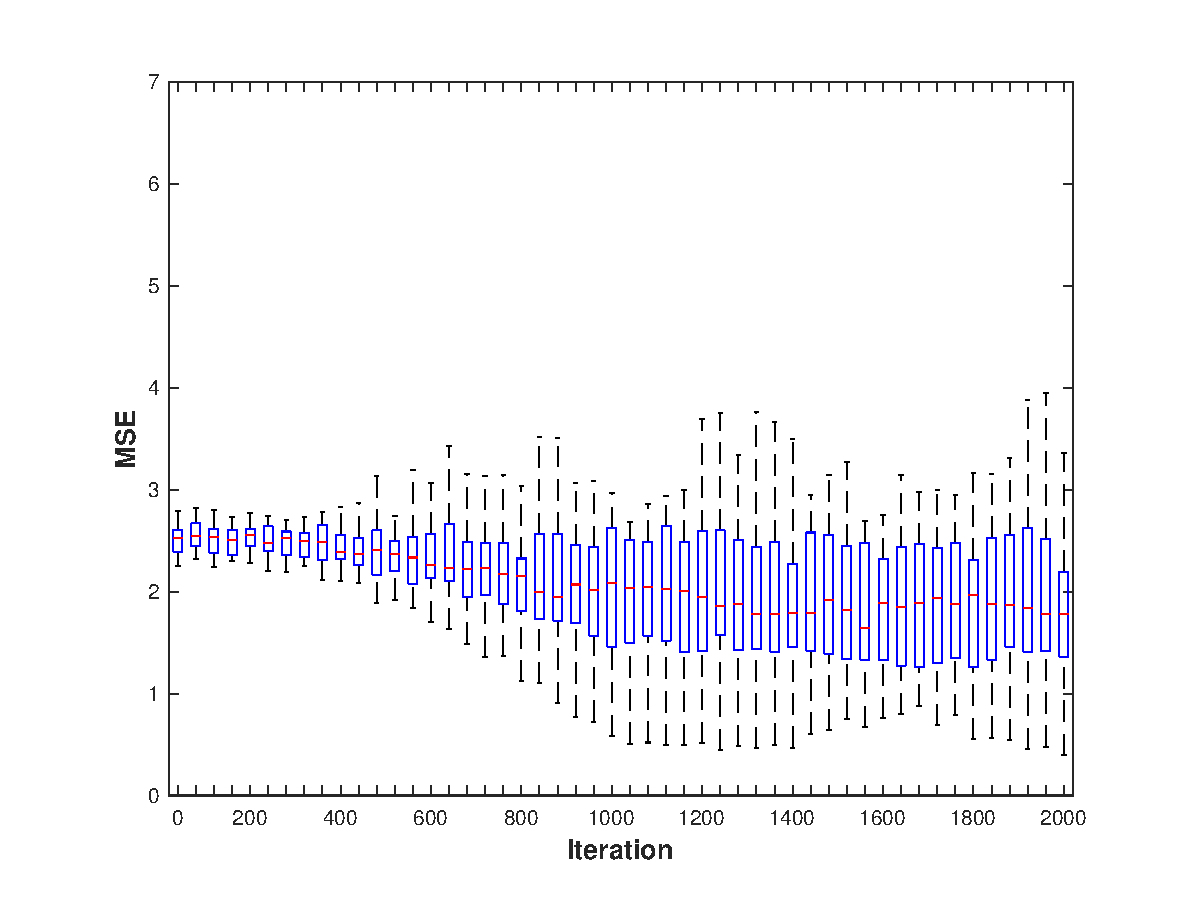
\includegraphics[width=5.5cm]{mse1.eps}
}
\quad
\subfigure[group 2]{
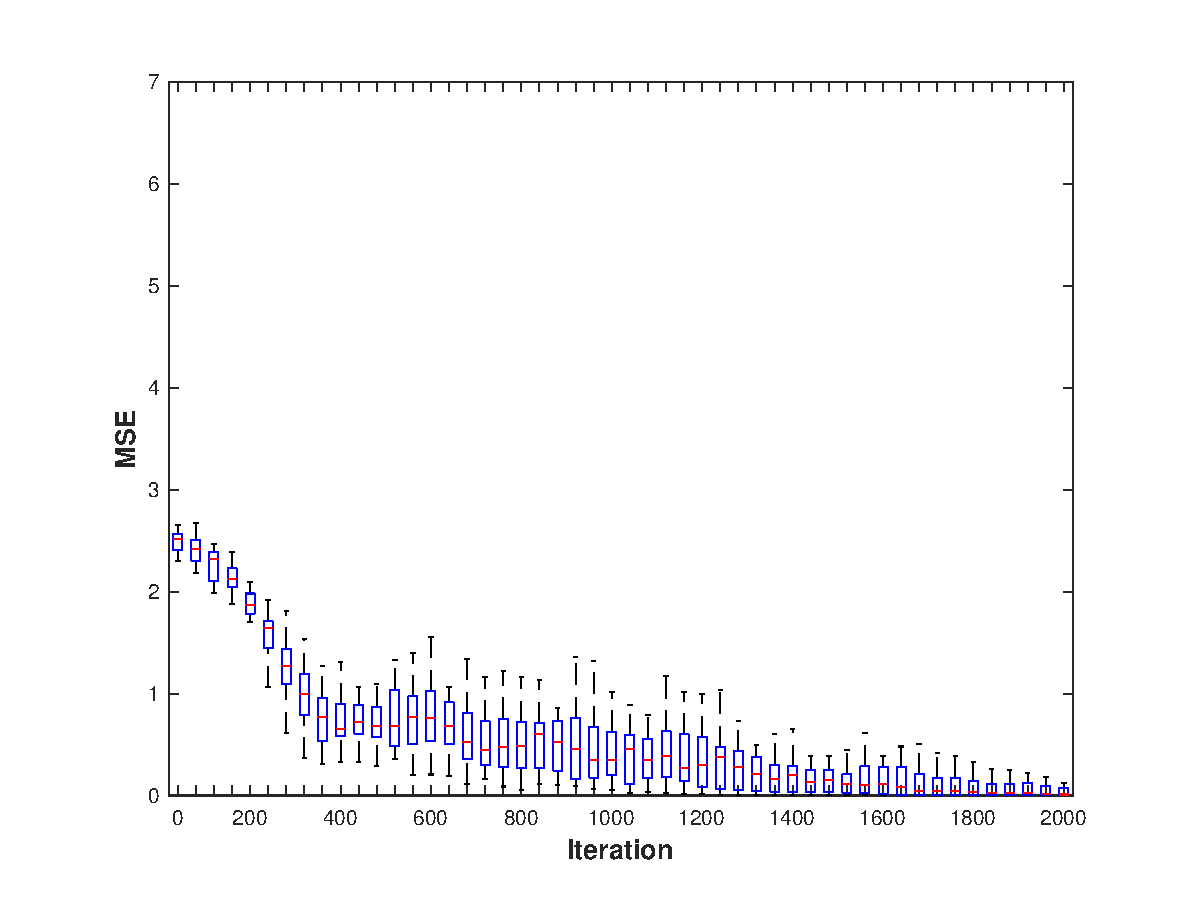
\includegraphics[width=5.5cm]{mse2.eps}
}
\quad
\subfigure[group 3]{
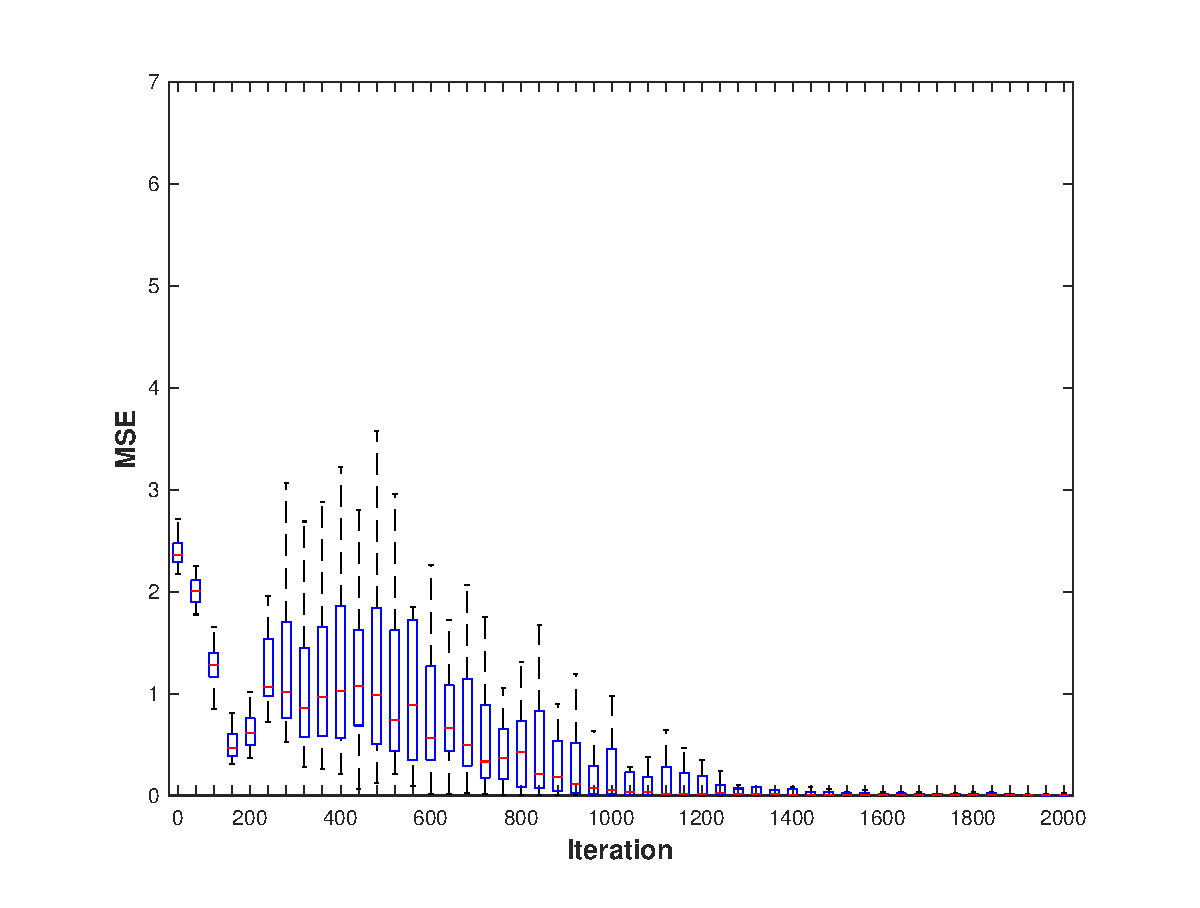
\includegraphics[width=5.5cm]{mse3.eps}
}
\quad
\subfigure[group 4]{
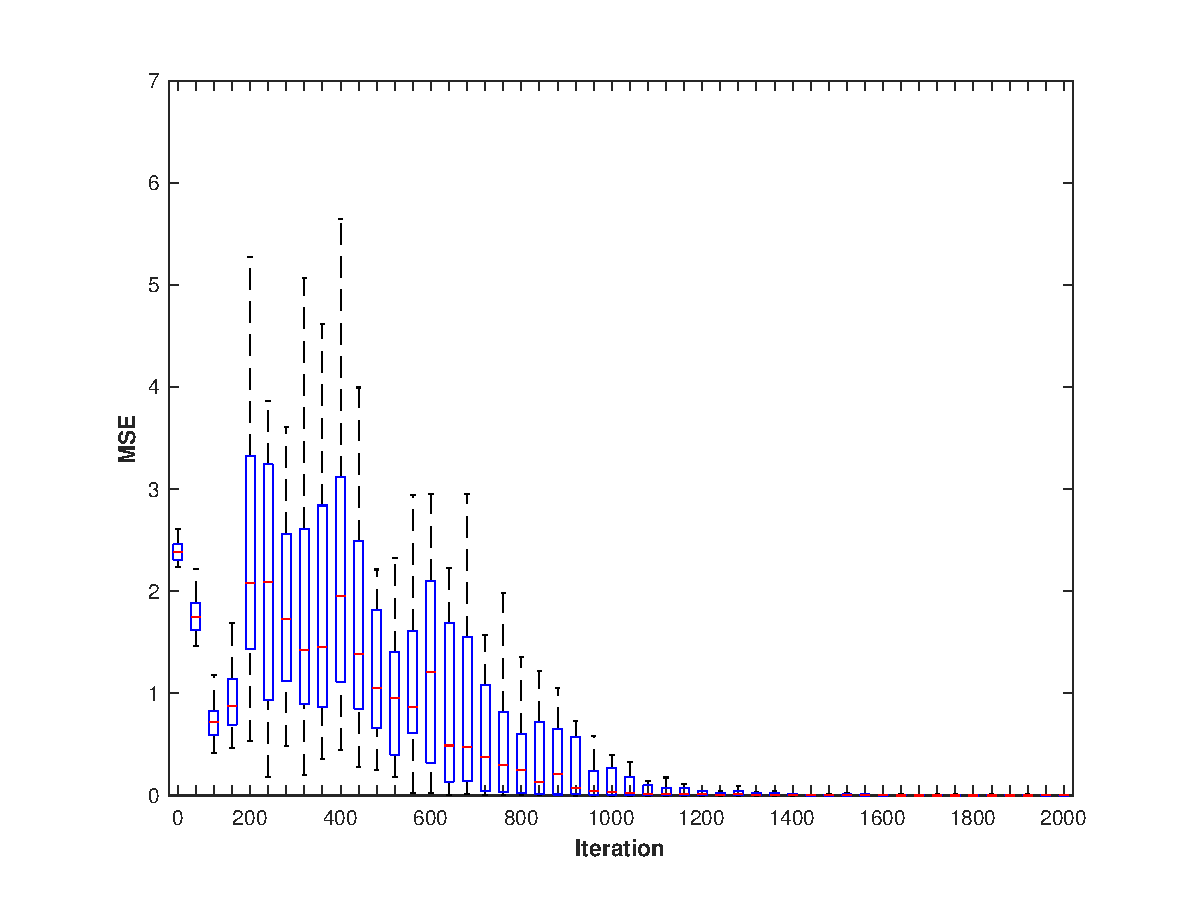
\includegraphics[width=5.5cm]{mse4.eps}
}
\caption{Result of experiment 1}
\label{fig: Result of experiment 1 }
\end{figure}
\\
In Figure 12, the x-coordinate of each subgraph represents the number of iterations, ranging from 0 to 2000; the y-coordinate is the value of MSE. Groups 1 to 4 respectively corresponds to subgraph (a) to subgraph (d). There was no significant decrease in MSE in subgraph (a), while in subgraph (b) there was a significant decrease, and when the training iterations reached 2000, the value of MSE just reached about 0.  For subgraph (c) and (d), when the training has not reached 2000 times, the value of MSE has fluctuated around 0.
\\
\newline
In order to observe the trend of MSE more clearly, we take the logarithm of MSE. According to the properties of the logarithm function, the logarithm function can scale the original part of MSE greater than 1, and enlarge the original MSE value within the range of 0 to 1, to see the slight fluctuation of the value more clearly. The logarithmic experimental results are shown in Figure 13.
\\
\begin{figure}[ht!]
\centering
\subfigure[group 1]{
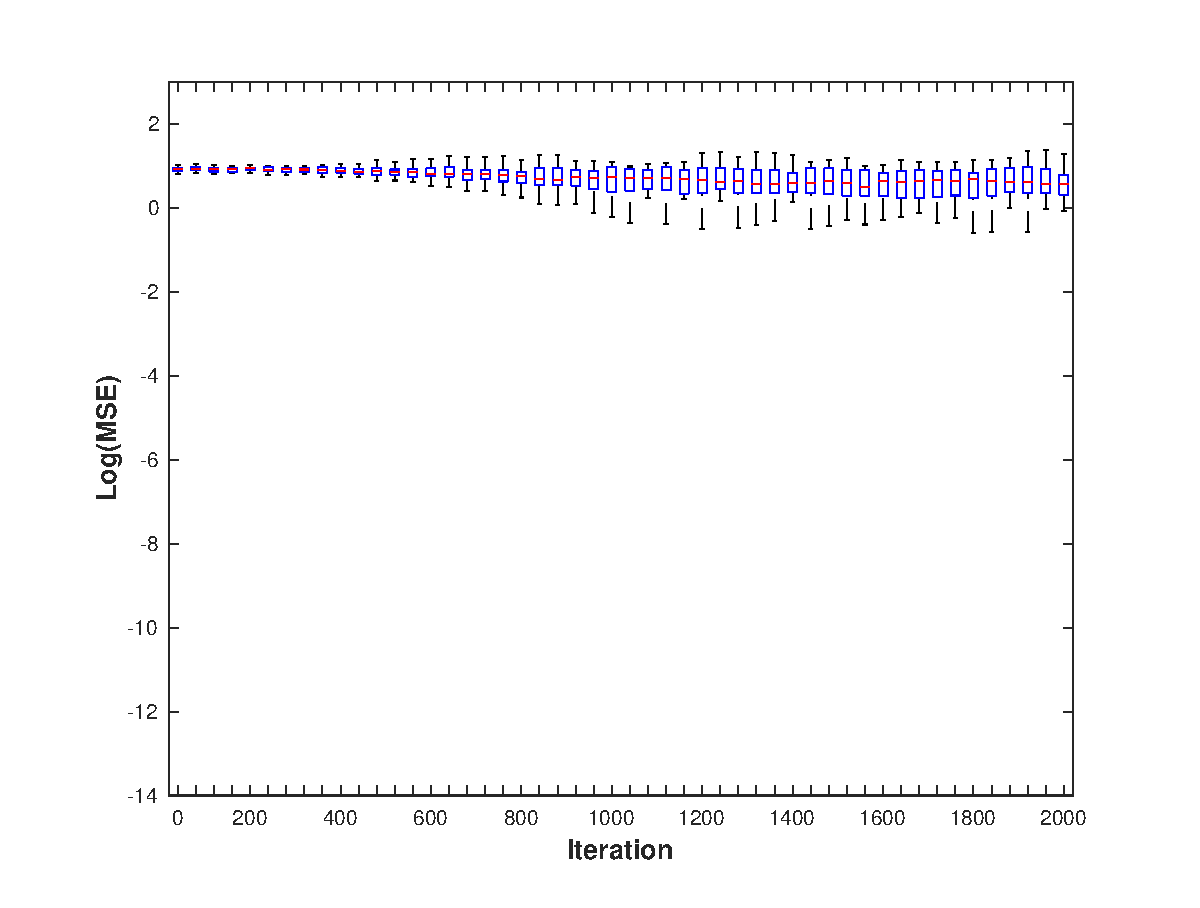
\includegraphics[width=5.5cm]{logmse1.eps}
}
\quad
\subfigure[group 2]{
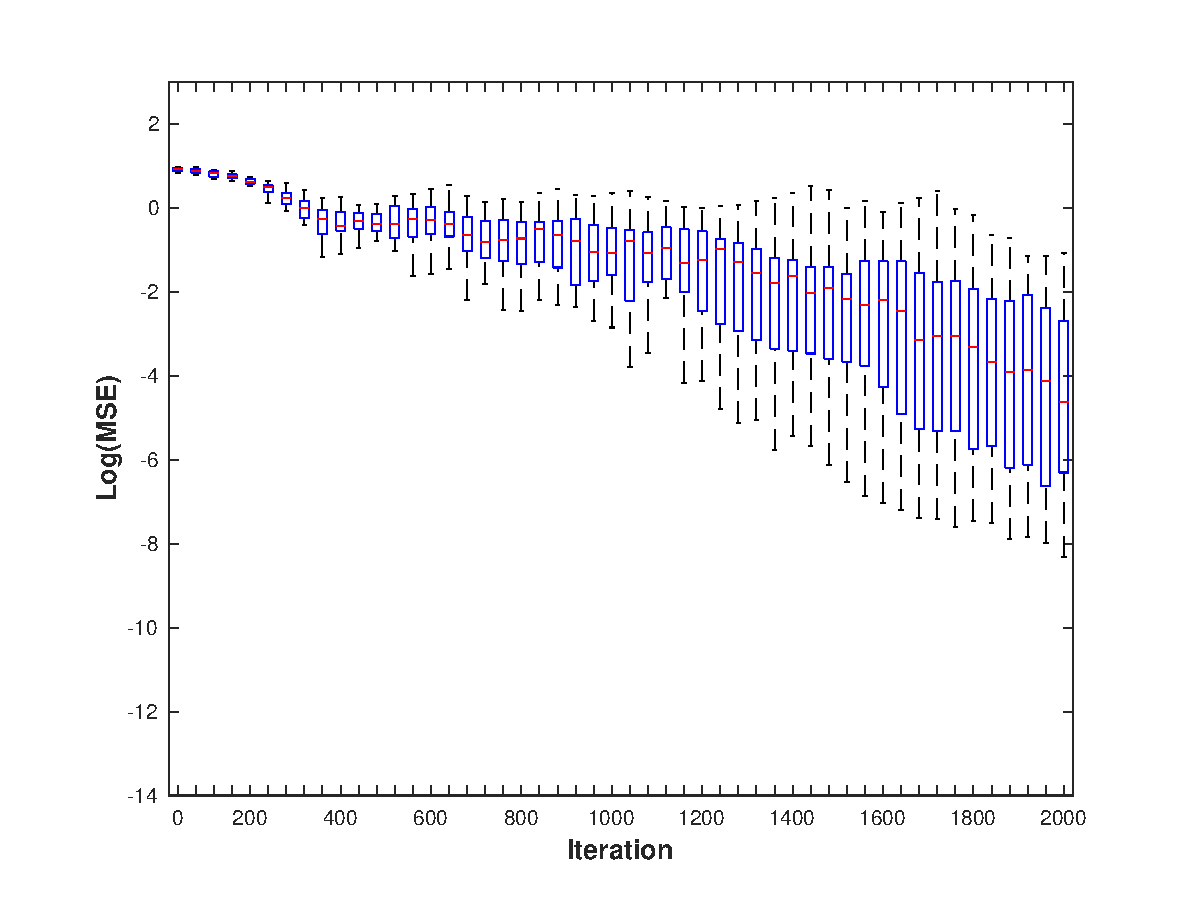
\includegraphics[width=5.5cm]{logmse2.eps}
}
\quad
\subfigure[group 3]{
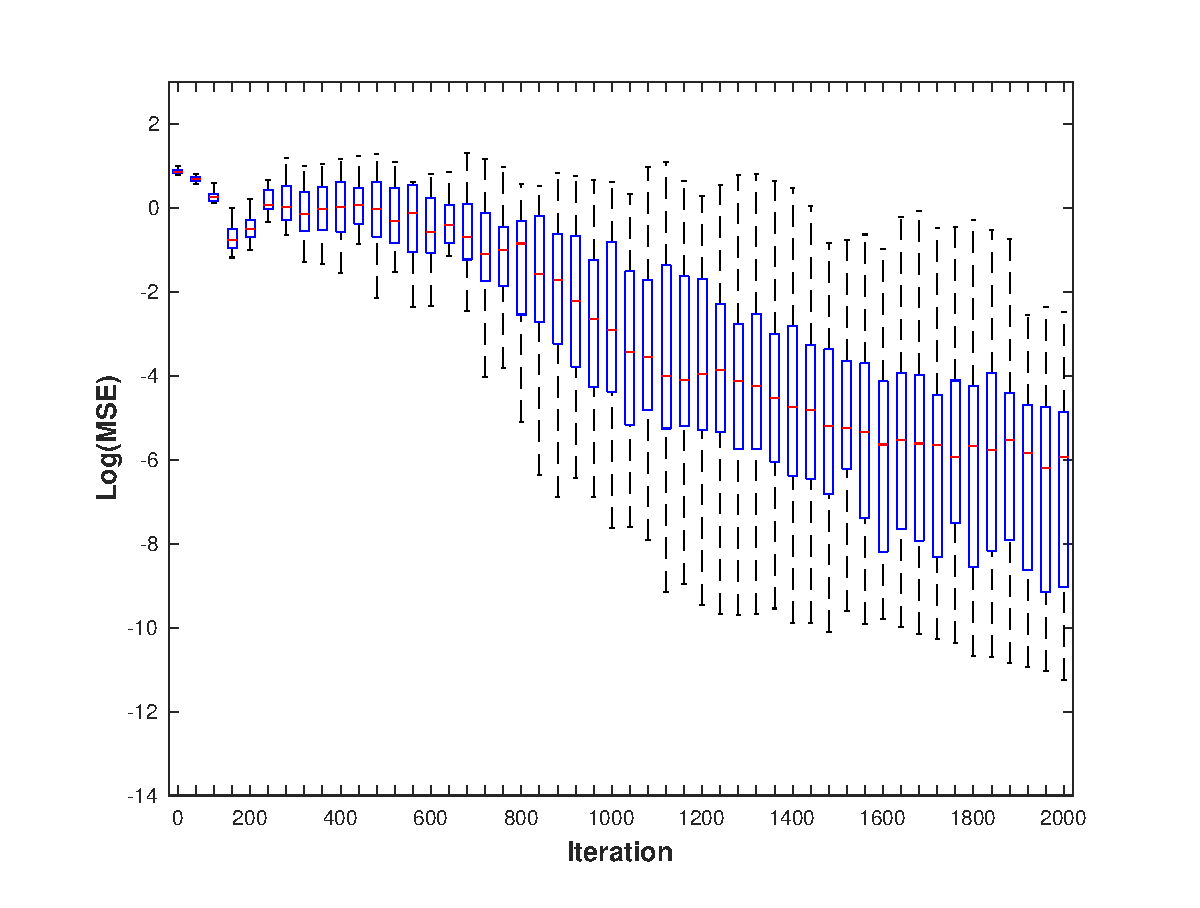
\includegraphics[width=5.5cm]{logmse3.eps}
}
\quad
\subfigure[group 4]{
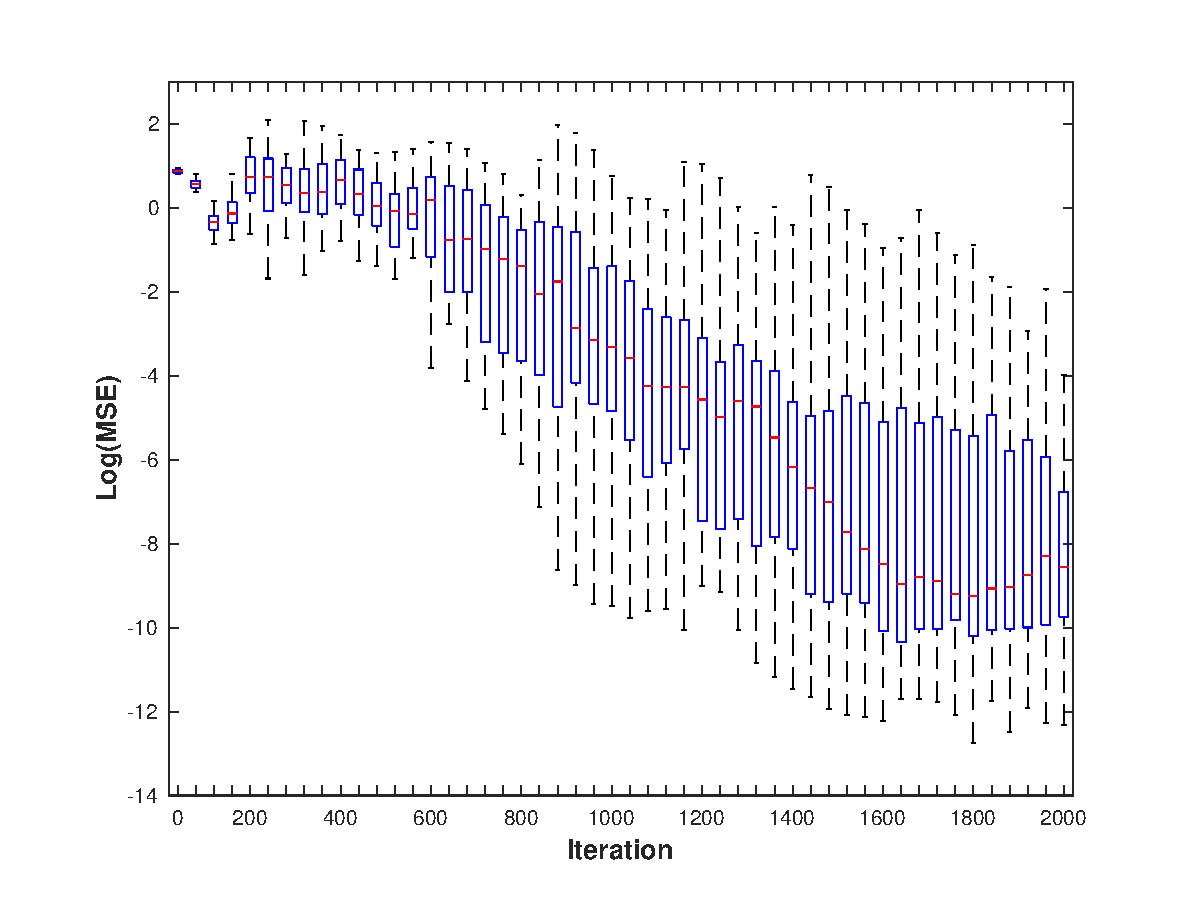
\includegraphics[width=5.5cm]{logmse4.eps}
}
\caption{Logarithmic MSE result of experiment 1}
\label{fig: Logarithmic MSE result of experiment 1}
\end{figure}
\\
In Figure 13, the x-coordinate of each subgraph represents the number of iterations, ranging from 0 to 2000; the y-coordinate is the logarithm of MSE. According to the trend of the box diagram in Figure 13, as the number of iterations in the training process increases, the logarithm of MSE value in subgraph (a) basically does not change, which indicates that the training effect of group 1 is not good, indicating that GAN cannot learn the state of dynamical system well and make correct predictions when the number of neurons is small. In subgraph  (b), (c) and (d), the logarithm of MSE value decreased significantly, and from the position of the median, the logarithm of MSE value of group 4 reached a plateau at the later stage of training, indicating that GAN's learning and prediction ability performed better under the neurons number setting of group 4.
\newpage
\subsubsection{Number of hidden layers}
After the first set of experiments, we can preliminarily think that 128 neurons in the hidden layer in the generator and discriminator neural networks will have a good training result. In addition to the number of neurons, the number of hidden layers also affects the training effect of the neural network. We fixed 128 neurons and divided them into different hidden layers for the next experiment.
\\
\newline
\begin{table}[ht]
\caption{Different number of hidden layers}
\vspace*{10pt}
\begin{tabular}{l|l|c|c|c|c}
\hline
                                                    &                                                             & \multicolumn{1}{l|}{Group 1}                            & \multicolumn{1}{l|}{Group 2}                                  & \multicolumn{1}{l|}{Group 3}                                        & \multicolumn{1}{l}{Group 4}                                               \\ \hline
Generator                                           & \begin{tabular}[c]{@{}l@{}}Input\\ ReLU\end{tabular}        & 2                                                       & 2                                                             & 2                                                                   & 2                                                                         \\
                                                    & Dense ReLU                                                  & \begin{tabular}[c]{@{}c@{}}128\\ 128\end{tabular}       & \begin{tabular}[c]{@{}c@{}}128\\ 128\\ 128\end{tabular}       & \begin{tabular}[c]{@{}c@{}}128\\ 128\\ 128\\ 128\end{tabular}       & \begin{tabular}[c]{@{}c@{}}128\\ 128\\ 128\\ 128\\ 128\end{tabular}       \\
                                                    & Output                                                      & 2                                                       & 2                                                             & 2                                                                   & 2                                                                         \\ \hline
\multicolumn{1}{c|}{\multirow{4}{*}{Discriminator}} & \begin{tabular}[c]{@{}l@{}}Input\\ Leaky ReLU\end{tabular}  & 4                                                       & 4                                                             & 4                                                                   & 4                                                                         \\
\multicolumn{1}{c|}{}                               & \begin{tabular}[c]{@{}l@{}}Dense \\ Leaky ReLU\end{tabular} & \begin{tabular}[c]{@{}c@{}}128\\ 128\\ 128\end{tabular} & \begin{tabular}[c]{@{}c@{}}128\\ 128\\ 128\\ 128\end{tabular} & \begin{tabular}[c]{@{}c@{}}128\\ 128\\ 128\\ 128\\ 128\end{tabular} & \begin{tabular}[c]{@{}c@{}}128\\ 128\\ 128\\ 128\\ 128\\ 128\end{tabular} \\
\multicolumn{1}{c|}{}                               & \begin{tabular}[c]{@{}l@{}}Dense\\ Leaky ReLU\end{tabular}  & 4                                                       & 4                                                             & 4                                                                   & 4                                                                         \\
\multicolumn{1}{c|}{}                               & \begin{tabular}[c]{@{}l@{}}Output\\ sigmoid\end{tabular}    & 1                                                       & 1                                                             & 1                                                                   & 1                                                                         \\ \hline
\end{tabular}
\label{table:Different number of hidden layers}
\end{table}
\\
The second set of experiments is to observe the effect of the number of hidden layers on GAN performance by changing the number of hidden layers when the number of neurons in the hidden layers of generator and discriminator is the same. In this experiment, there are four experimental groups, and the specific settings of hidden layers of the four experimental groups are shown in Table 2. Same like the previous experiment, each group of experiments was repeated for 20 times. For each experiment, we set the number of iterations of training to be 2000 and recorded the MSE value every 40 iterations. Through 20 repeated experiments, a box diagram was drawn to observe the trend of GAN performance during the training process. From the experience of the previous experiment, if MSE box graph is drawn directly, in the later training period, MSE is likely to be close to 0, and its trend is difficult to observe. Therefore, we take the logarithm of all MSE values again and then draw box graph, and the result is shown in Figure 14.
\\
\newline
\begin{figure}[ht!]
\centering
\subfigure[group 1]{
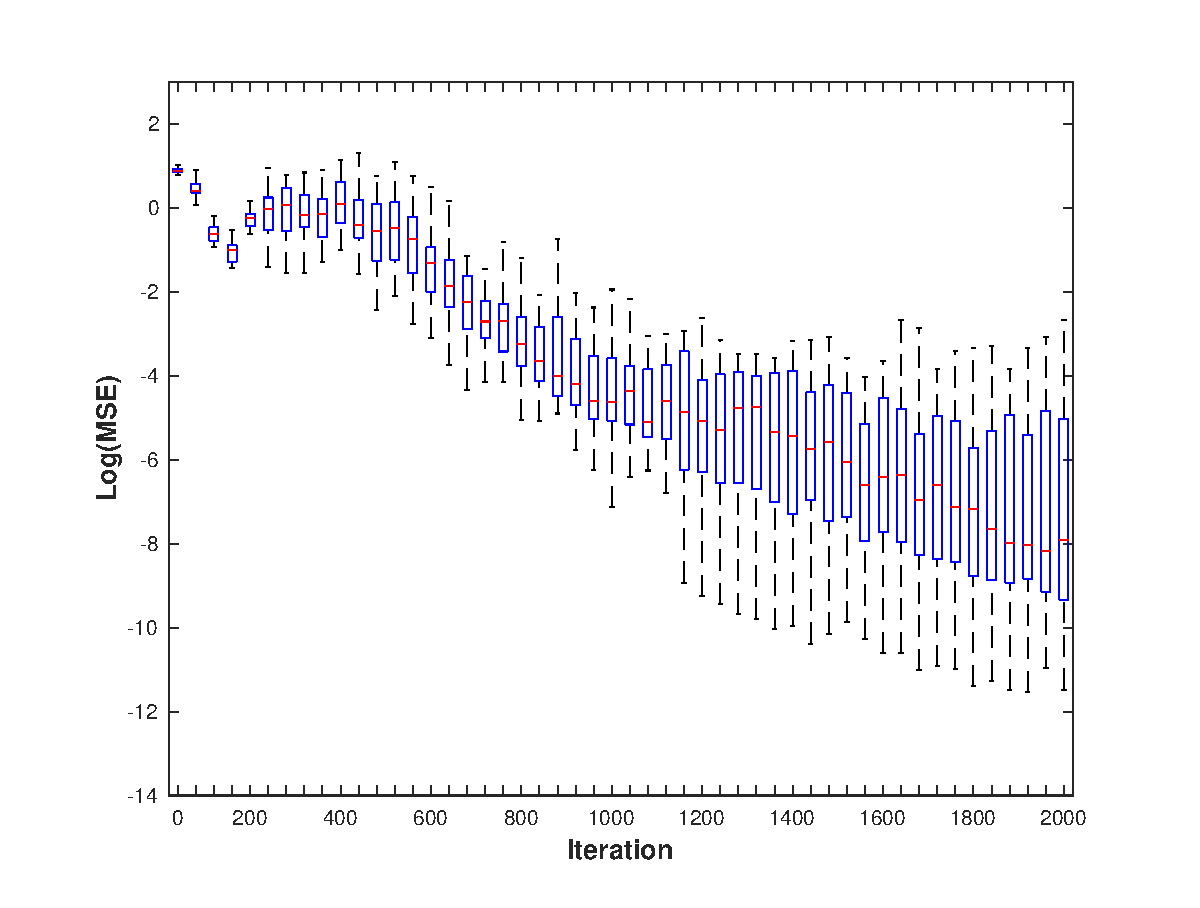
\includegraphics[width=5.5cm]{logmse5.eps}
}
\quad
\subfigure[group 2]{
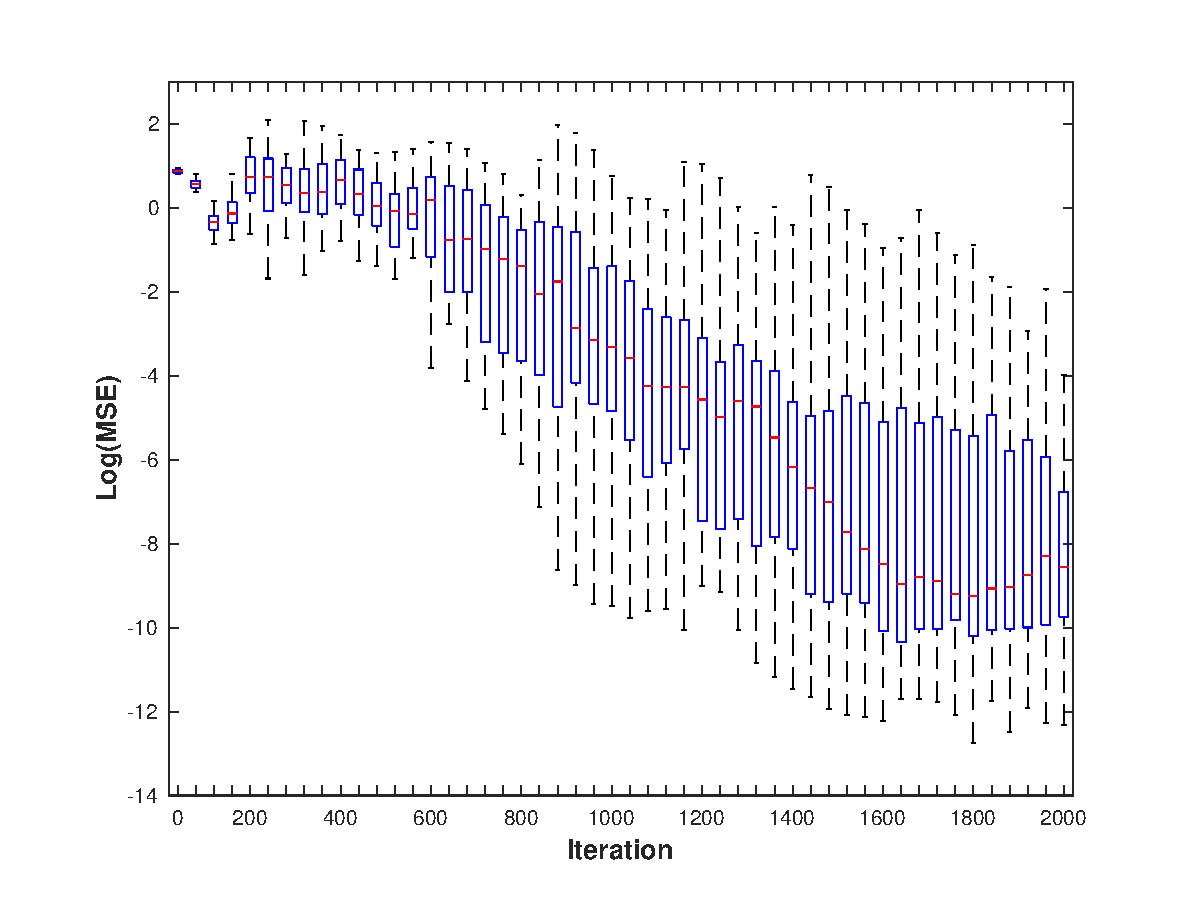
\includegraphics[width=5.5cm]{logmse4.eps}
}
\quad
\subfigure[group 3]{
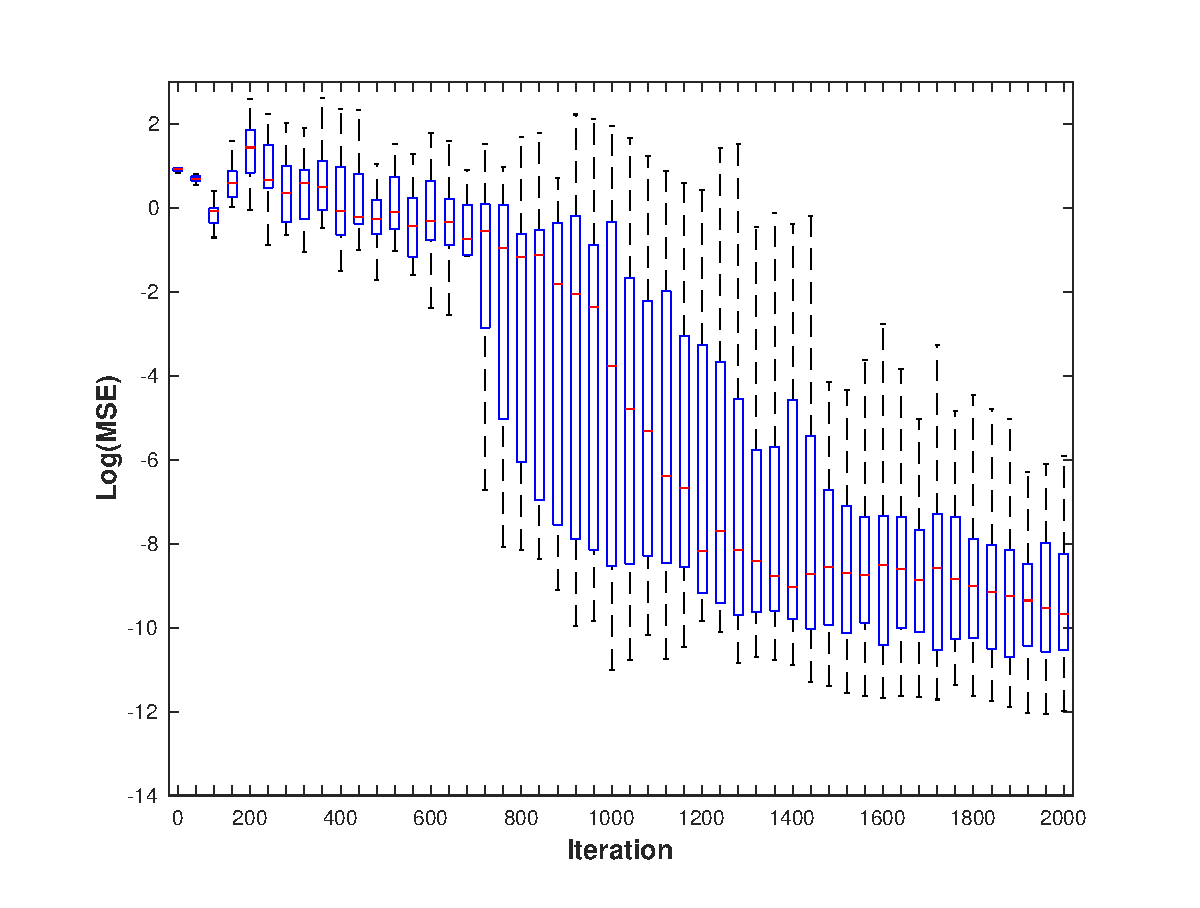
\includegraphics[width=5.5cm]{logmse6.eps}
}
\quad
\subfigure[group 4]{
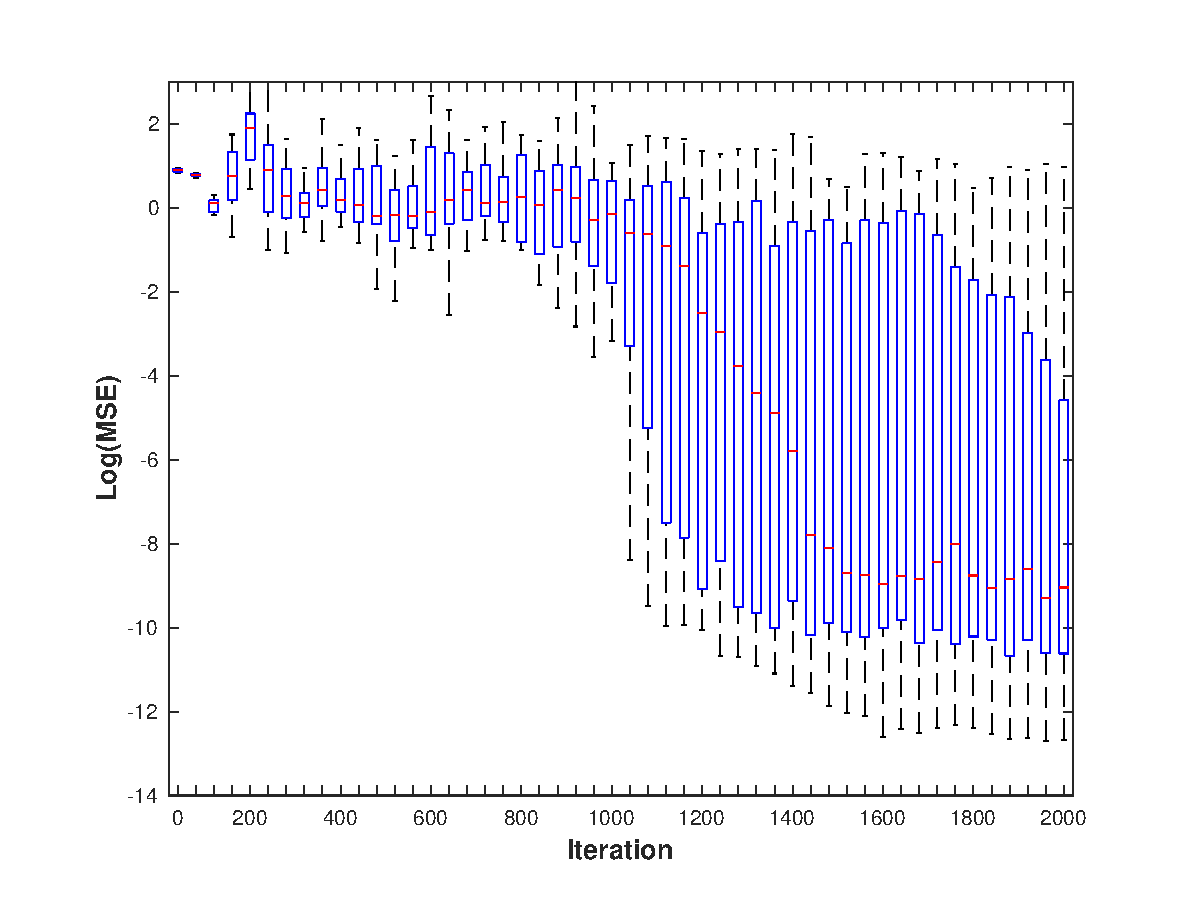
\includegraphics[width=5.5cm]{logmse7.eps}
}
\caption{Logarithmic MSE result of experiment 2}
\label{fig: Logarithmic MSE result of experiment 2}
\end{figure}
\\
In Figure 14, the x-coordinate of each subgraph represents the number of iterations, ranging from 0 to 2000; the y-coordinate is the logarithm of MSE. Groups 1 to 4 respectively corresponds to subgraph (a) to subgraph (d). From the declining trend of the median of the box graph and the range of the quartile of the box graph, the MSE value of group 1 corresponding to subgraph (a) is always in the declining stage, which indicates that GAN training has not reached a stable stage when the training times reach 2000. It shows that if the hidden layers of generator and discriminator are too few, training efficiency will be affected and training efficiency will be slowed down. In group 2 corresponding to subgraph (b), MSE is close to 0 and tends to be stable at the later stage of training. However, compared with group 3 corresponding to subgraph (c), the training of group2 is stable at the later stage, but the quartile range of box graph shows that group 2 is not as stable as group 3 at the later stage of training, and the MSE of group 3 has prominent descending stage and stable stage, and the fluctuation range is small, so we can consider that the training effect of group3 is better. For group 4 corresponding to subgraph (d), in the second half of the training, although the median value tends to be stable, the quartile range of the box graph even occupies the entire y-axis, which indicates that GAN's performance does not tend to be stable at the later stage of training, but has higher volatility. Based on this result, we can preliminarily believe that for the current problem, if too much hidden layer is added in generator and discriminator, the training effect will not be improved, and on the contrary, the training will become unstable, or overfitting phenomenon will occur.
\\
\newline
Based on the above phenomena, we can conclude that appropriately increasing the number of hidden layers of generator and discriminator will help GAN training, but if too many hidden layers are added, GAN training will become unstable. In this set of experiments, GAN showed better learning and prediction ability under the hidden layer number setting of group 3.
\newpage
\subsection{Different training iterations}
After the above two sets of experiments, we know that in the neural network of generator and discriminator, the number of neurons in the hidden layer and the number of hidden layers have certain influence on the training of GAN. GAN should have a specific predictive ability after learning the existing dynamic system state. In GAN, input a state to the generator, and the generator will output a predicted value, the discriminator then distinguishes the output of the generator. After GAN has been trained, the generator model is saved, an initial input state is given to the generator, and the output of the generator is used as the input of the next generator with the idea of loop iteration. After a certain number of iterations, the generator should be able to predict the next set of states based on one input state.
\\
\newline
In order to observe the predictive ability of the generator after different training times, we selected the most effective setting of the two groups of experiments above, continued to use the single pendulum model, and then saved different generator network models under different training iterations. We graph the states predicted by the generator. The standard motion state of a single pendulum is shown in chapter 3.
\\
\newline
\begin{figure}[ht!]
\centering
\subfigure[500 iterations]{
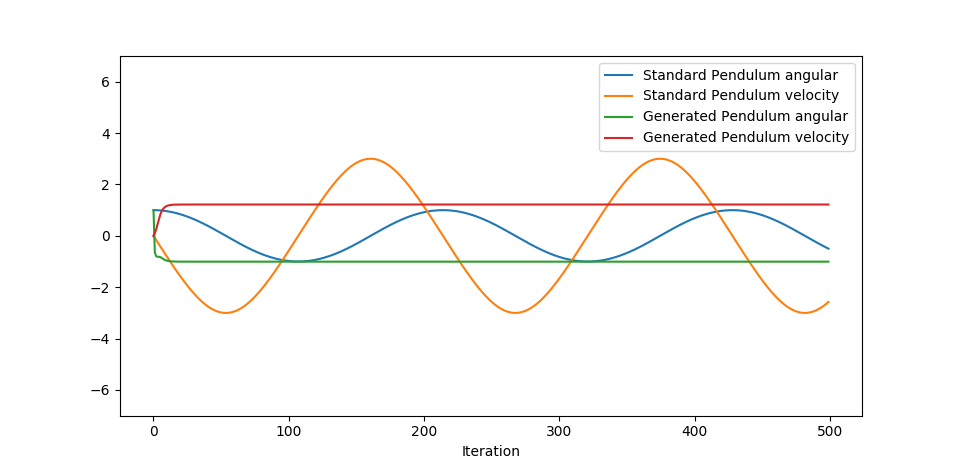
\includegraphics[width=5.5cm]{pendulum_500.png}
}
\quad
\subfigure[1000 iterations]{
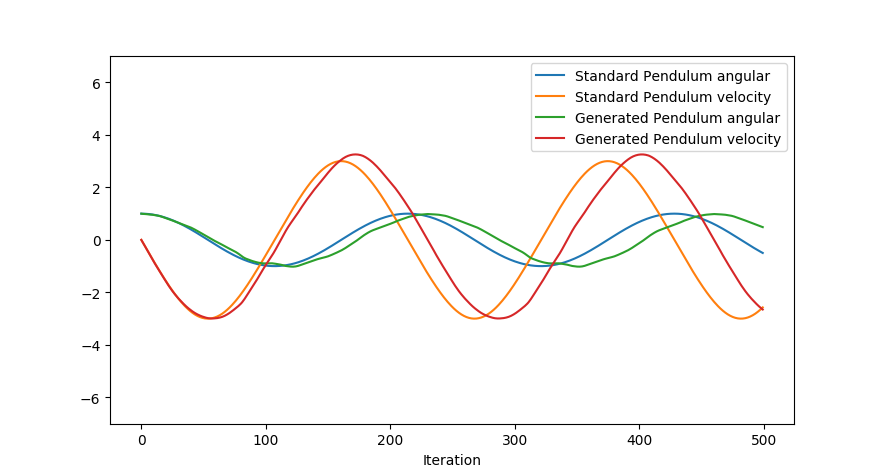
\includegraphics[width=5.5cm]{pendulum_1000.png}
}
\quad
\subfigure[1500 iterations]{
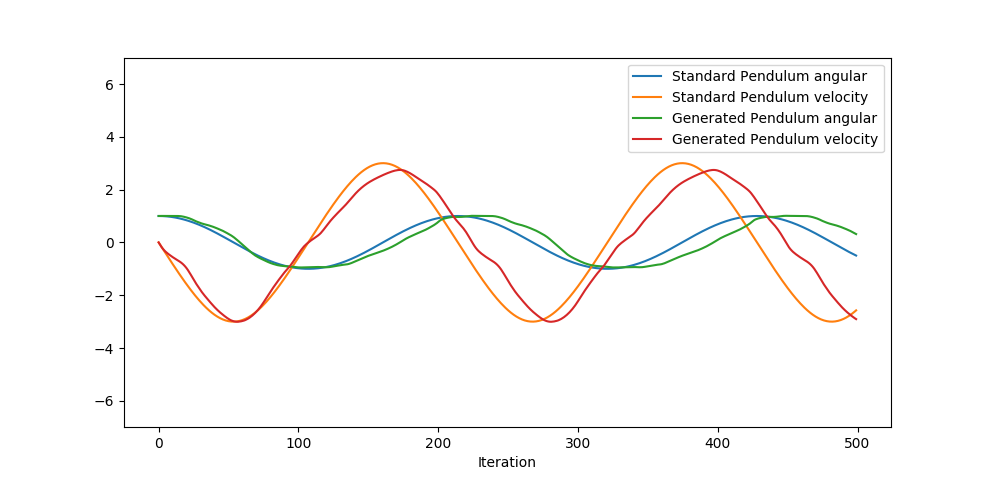
\includegraphics[width=5.5cm]{pendulum_1500.png}
}
\quad
\subfigure[2000 iterations]{
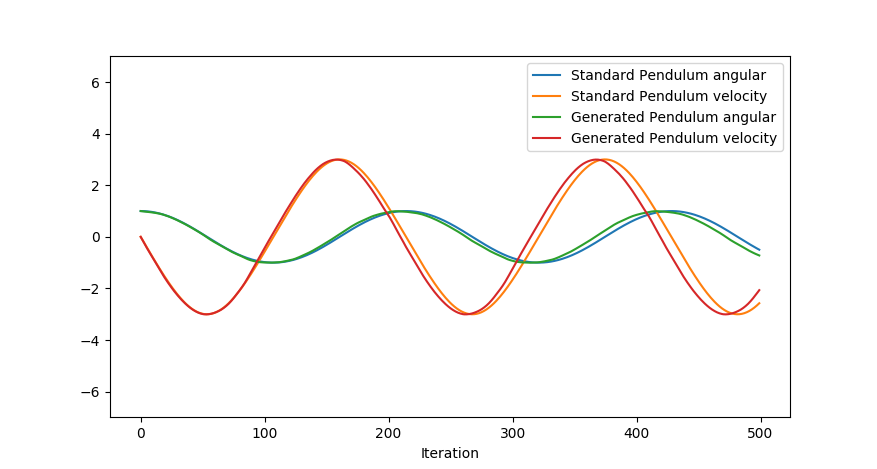
\includegraphics[width=5.5cm]{pendulum_2000.png}
}
\caption{Different training iterations}
\label{fig: Different training iterations}
\end{figure}
\\
The four subgraphs of Figure 15 respectively correspond to the initial single pendulum state of the generator when the training iterations are 500,1000,1500 and 2000, and the track of the single pendulum state predicted by the generator. In each subgraph, the blue line represents the swing angular of the standard single pendulum, the yellow line represents the swing velocity of the standard single pendulum, the green line represents the swing angular of the single pendulum generated by the generator, and the red line represents the swing velocity of the single pendulum generated by the generator. As can be seen from the changes of the four subgraphs, with the increase of training iterations, the state generated by the generator and the standard state is more and more fitted. Of course, in each iteration, as the number of iterations increases, the errors accumulate. There will be a deviation between the predicted state track and the standard state track in the later iteration.
\subsection{Result}
Through the experiments in the above two parts, we know that the topological structure of GAN will have an impact on the training effect, and enough training iterations are needed to make GAN achieve a good prediction effect. We select the above well-behaved parameter settings and initialize the state of the single pendulum and double pendulum and input the initial state into the pre-trained generator model respectively, and the following prediction results can be obtained. Visualization of the prediction of the single and double pendulum has been shown in the demonstration. In the dissertation, we show the track curves of the motion states of the single and double pendulum.
\\
\begin{figure}[h!]
\centering
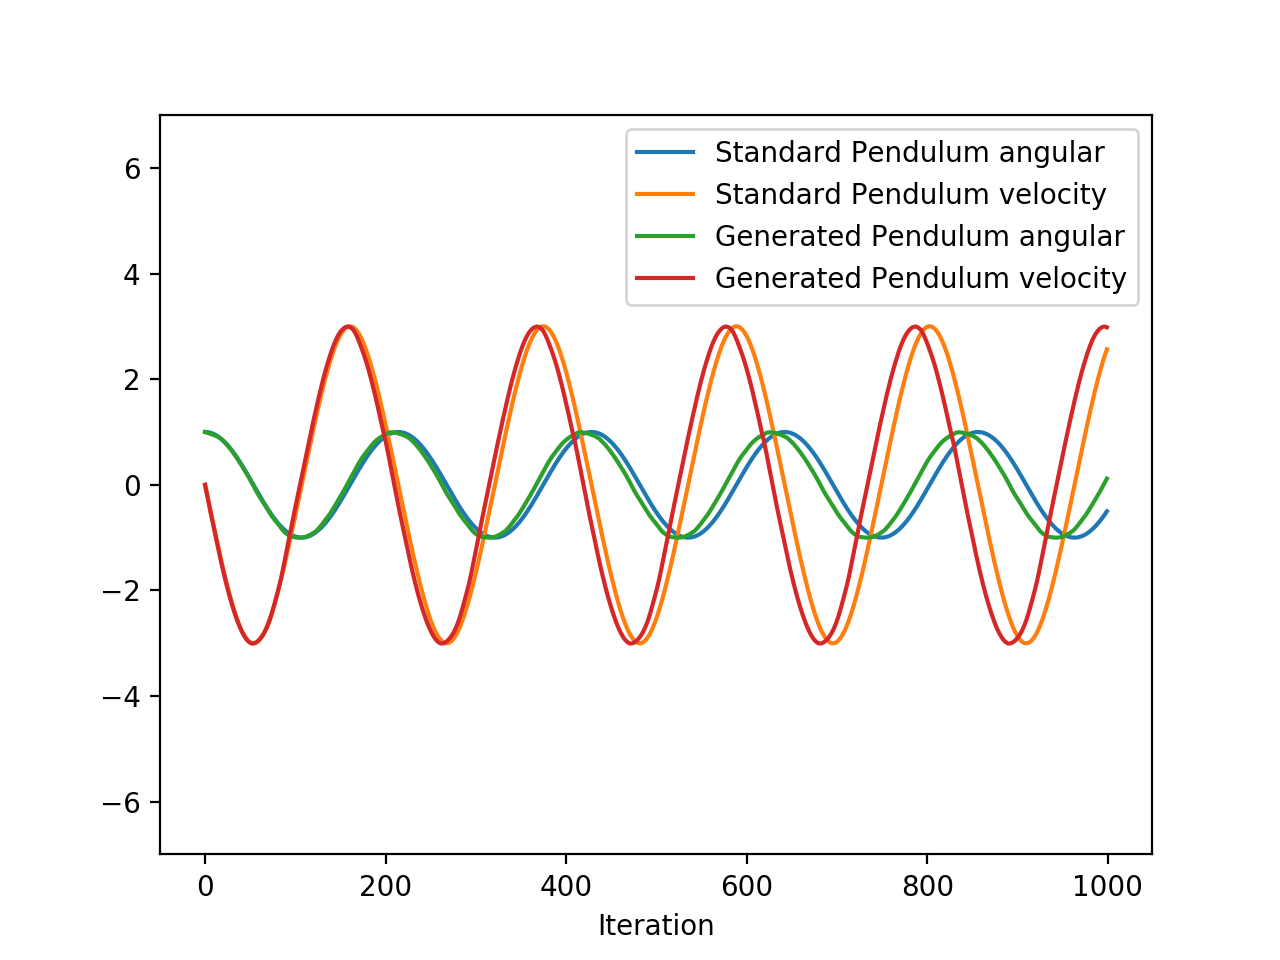
\includegraphics[scale=0.6]{12.png}
\caption{Single pendulum track}
\label{fig:Single pendulum track}
\end{figure}
\begin{figure}[ht!]
\centering
\subfigure[Standard double pendulum track]{
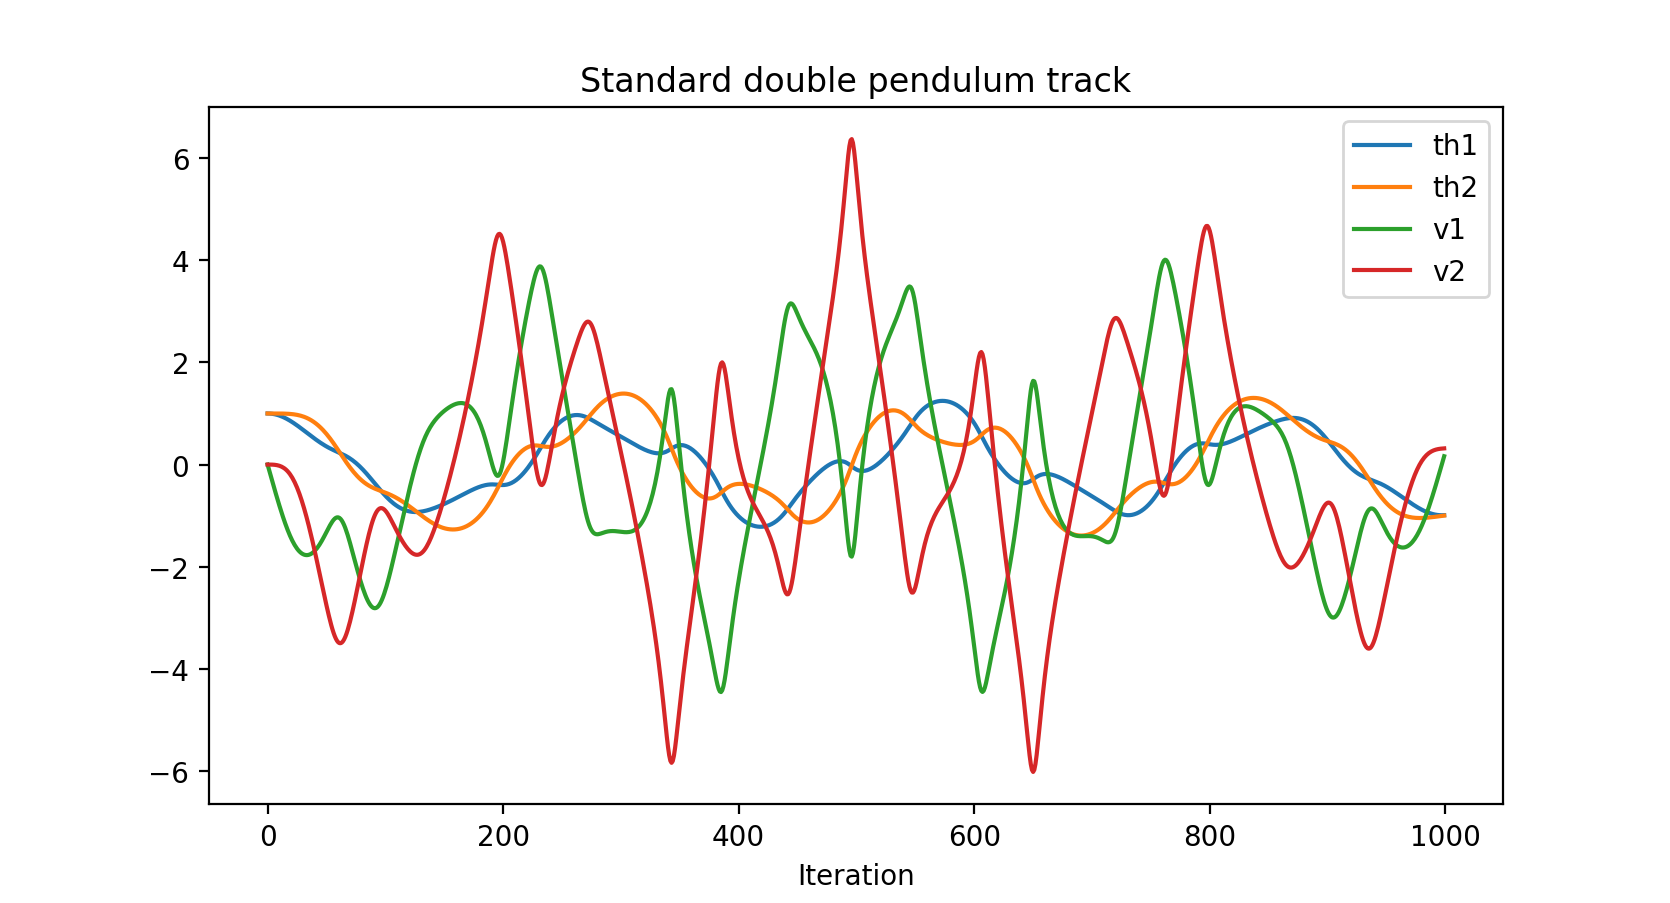
\includegraphics[width=10cm]{13.png}
}
\quad
\subfigure[Generated double pendulum track]{
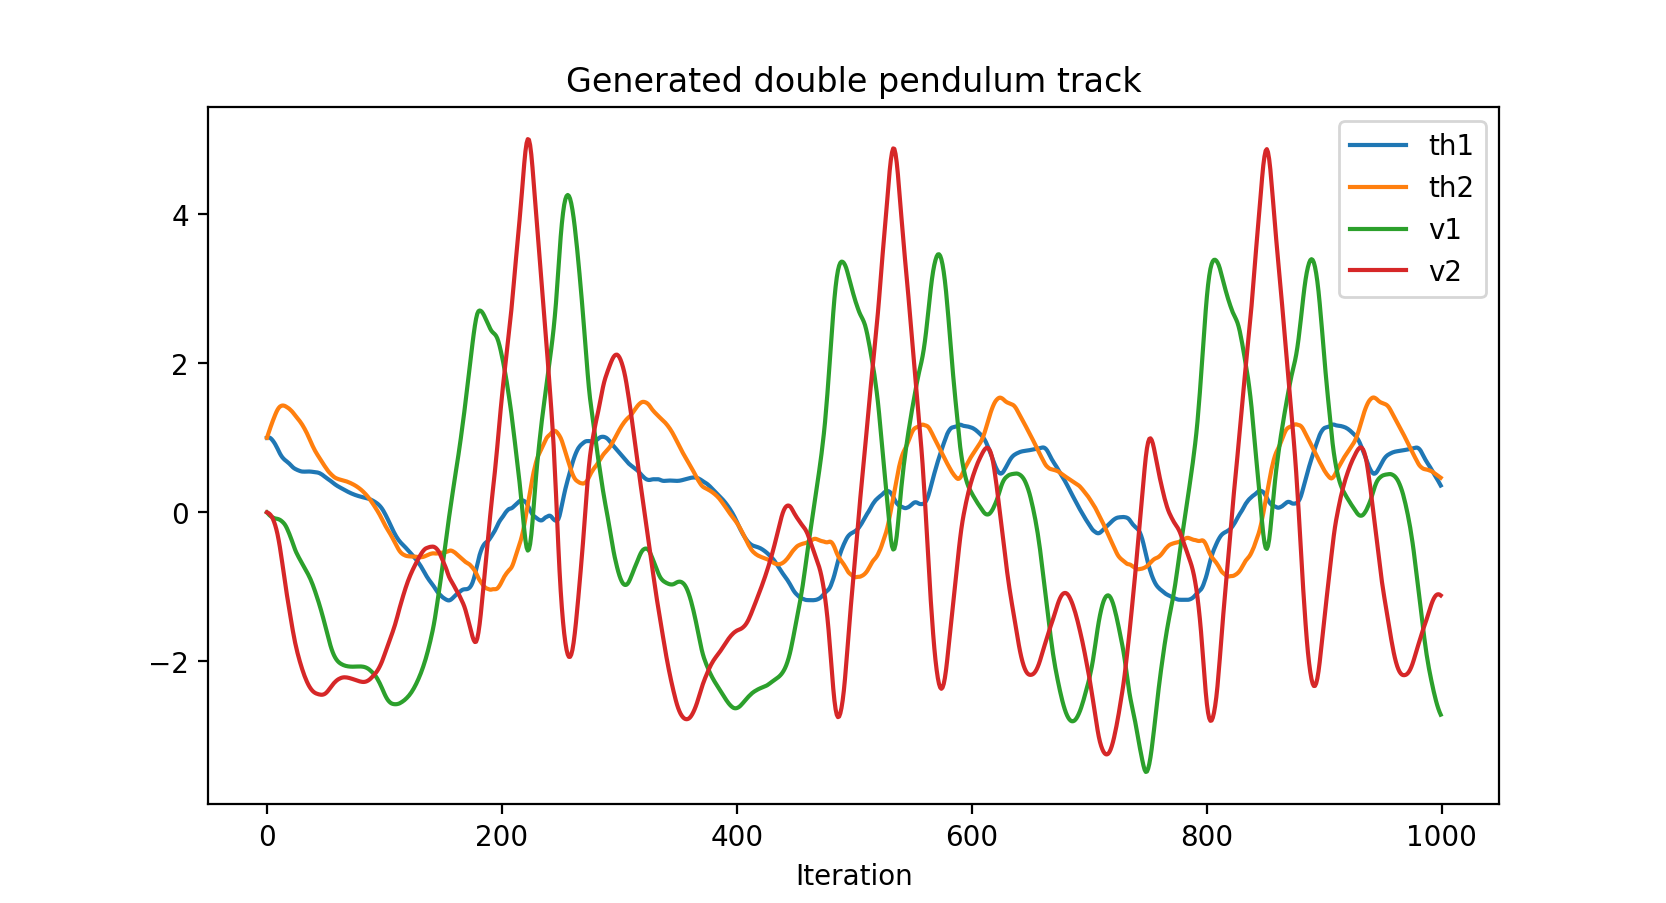
\includegraphics[width=10cm]{14.png}
}
\caption{Double pendulum track}
\label{fig: Double pendulum track}
\end{figure}
\\
In Figure 16, the blue line represents the swing angular of the standard single pendulum, the yellow line represents the swing velocity of the standard single pendulum, the green line represents the swing angular of the single pendulum generated by the generator, and the red line represents the swing velocity of the single pendulum generated by the generator.
\\
\newline
In Figure 17, the subgraph (a) represents the curve of the motion state of the standard double pendulum, the subgraph (b) represents the curve of the motion state of the generated double pendulum predicted by generator. The blue line represents the swing angular of ball 1, the yellow line represents the swing angular of ball 2, the green line represents the swing velocity of ball 1, and the red line represents the swing velocity of ball 2.

\newpage
\section{Discussion}
The last chapter mainly introduces two groups of experiments and experimental results. The first group of experiments is about the influence of topological structure on GAN training, and the influence of different training iterations on GAN prediction ability in the second group of experiments. In the first set of experiments, we set up control experiments from the number of neurons in the hidden layer and the number of hidden layers to observe the performance of GAN under different network topologies. In the experiment on the number of neurons, we get the result that if the number of neurons is set too small, such as group1, the number of neurons in the hidden layer is 4 and 16 respectively, GAN training does not affect. When the hidden layer neurons of each layer are set at 128, GAN training has the prominent descending stage and stable stage, and the training effect is good. However, if a simple dynamical system, such as a simple pendulum system, has a straightforward differential equation, it should not require too many neurons to fit the simple differential equation well, but the experimental results are not like this.Perhaps because the state of a dynamical system changes dynamically from moment to moment, it takes enough neurons to fit even a simple differential equation. Therefore, it can be inferred that for more complex systems, the behaviour of the state change will be more complex, and more neurons should be needed to achieve a better learning effect.
\\
\newline
In the experiment on the number of hidden layers, since we have set up enough neurons, GAN can learn even when the number of hidden layers is small, but the learning process is slow. As the number of layers increases, GAN's learning ability gradually improves, but the number of layers cannot be increased all the time. For example, group 4 in experiment 2, when the number of layers increases too much, the results of later training fluctuate considerably, and the phenomenon of over-fitting has likely occurred. The model trained in this way is not as good as the model trained when the number of layers is less. This experimental phenomenon also reflects the theory of the power of depth\citep{eldan2016power}, which means that the fitting effect of a neural network with two layers is never as good as that of a neural network with three layers. However, this theory does not mean that the number of layers of neural network should be infinite. We should choose the most suitable parameter settings with the highest efficiency, to improve the training efficiency and reduce the computational cost. In the above two groups of experimental results, there is a strange phenomenon in the curve of MSE drawn. The value of MSE will drop for a period of time, then rise suddenly, and then decline slowly until it is stable. There is still no reasonable explanation for this problem, which is also a problem worth further study.
\\
\newline
After the experiment, we select the good parameters and train the generator model, and then give the generator an initial state and let the generator make the cyclic prediction. The prediction result of the single pendulum is good, but it will accumulate a little deviation as the number of iterations increases, and the overall motion state and trajectory remain unchanged. By contrast, the prediction result of the double pendulum is not as good as that of the single pendulum. It may be because the motion state of the two balls is too complicated, and a slight deviation will increase the subsequent impact. The generator has a weak prediction effect on the double pendulum, which is also a limitation of this project. Moreover, due to the tight time, we did not apply more models to test GAN's prediction ability, but only used the pendulum model. If there is more time for research, we will consider applying more different kinds of dynamical system models to verify GAN's prediction ability, which makes our conclusion more convincing. However, at least we can know that GAN can be used to predict the following states based on existing dynamic system states. What continues to be studied is whether other types of GAN can have better predictive ability.

\newpage
\section{Conclusion}
Through the above experiments and achieve the results. We can conclude that GAN can be used to predict the following states based on the existing states of dynamical systems. Through experiments, we can know that the number of neurons in the hidden layer and the number of hidden layers have an impact on GAN's training performance, and it is essential to select a suitable training parameter. In terms of the types of predicted dynamical systems, this project mainly tested two dynamical systems, single pendulum and double pendulum, which respectively represent simple and complex dynamical systems. It is shown in the prediction results that the generator is given an initial pendulum state by using the pre-trained GAN generator, the generator can well predict the following state based on this initial state, which is consistent with the calculation results of the differential equation. When the generator is used to predict the double pendulum system, although the prediction effect is not as good as that of the single pendulum, it also has an outstanding prediction ability, and the generated state conforms to a particular double pendulum swing law rather than chaos. In this project, pendulum system was used as an example of dynamical system for research, and good results were obtained, showing that GAN has the ability to be applied to predict the state of the dynamical system. Of course, more research needs to be improved.

\newpage
\bibliographystyle{hc-en}
\bibliography{references}
\newpage
\appendix
\section{Kullback–Leibler divergence}
Kullback–Leibler divergence (KLD) is also known as relative entropy, information divergence, information gain. KL divergence is an asymmetric measure of the difference between two probability distributions P and Q. KL divergence is used to measure the number of extra bits required to encode the average of samples from P using Q based codes. Typically, P represents the true distribution of data, Q represents the theoretical distribution, model distribution, or approximate distribution of P.
\\
\newline
For discrete random variables, the KL divergence of probability distribution P and Q can be defined as:
\\
$$
D_{\mathrm{KL}}(P \| Q)=-\sum_{x \in \mathcal{X}} P(x) \log \left(\frac{Q(x)}{P(x)}\right)
$$
\\
which is equivalent to
$$
D_{\mathrm{KL}}(P \| Q)=\sum_{x \in \mathcal{X}} P(x) \log \left(\frac{P(x)}{Q(x)}\right)
$$
\\
Because the logarithm function is convex, the value of KL divergence is not negative\citep{cover2012elements}.
\section{Jensen–Shannon divergence}
Jensen–Shannon divergence (JSD) measures the similarity of two probability distributions, also known as Information radlus (IRad). JS divergence is a variant of KL divergence, which solves the problem of asymmetric KL divergence. In general, JS divergence is symmetric, and its value is between 0 and 1. The definition is as follows:
\\
$$
\operatorname{JSD}(P \| Q)=\frac{1}{2} D(P \| M)+\frac{1}{2} D(Q \| M)
$$
\\
where $
M=\frac{1}{2}(P+Q)
$\citep{cover2012elements}.
\section{Source Code}
All implementation codes of this project can be found on school gitlab account:
\\
\textit{https://git-teaching.cs.bham.ac.uk/mod-msc-proj-2018/bxz858}
\\
Compiling environment:
\\
\textit{Python 3.6.7rc2}
\\
\textit{PyTorch 1.1.0.post2}
\\
\newline
In the source code, \textit{pendulum4.py} and \textit{double\_pendulum.py} are respectively to train GAN to learn single pendulum and double pendulum. \textit{load\_pendulum.py} and \textit{load\_double\_pendulum.py} respectively give the trained generator of GAN an initial state to predict the following state, and the code also contains the visualization part.
\\
\newline
In the simple pendulum and double pendulum state generated part, reference the \textit{HYRY Studio} written \textbf{Use Python do scientific computing}, the site is \textit{http://bigsec.net/b52/scipydoc/double\_pendulum.html}
\end{document}
